\documentclass[10pt]{article}
\usepackage[T1]{fontenc}
\usepackage[utf8]{inputenc}
\usepackage[margin=0.8in]{geometry}
\usepackage{amsmath}
\usepackage{booktabs}
\usepackage{longtable}
\usepackage{array}
\usepackage{graphicx}
\usepackage{placeins}
\usepackage{hyperref}
\graphicspath{{figures/}{overleaf_trace_features/figures/}}

\title{Trace Features for Machine Learning:\\ the Complete List (\texttt{trace\_features.py})}
\author{ML-assisted optimization of CCD operating parameters --- working note}
\date{9 October 2026; updated 22 October 2026}
\newcommand{\code}[1]{\texttt{#1}}
% long feature names and paths in typewriter type: allow line breaks after underscores and slashes
\let\oldunderscore\_
\renewcommand{\_}{\oldunderscore\allowbreak}
\setlength{\emergencystretch}{3em}

\begin{document}
\maketitle

\begin{abstract}
This note lists every feature computed from one raw skipper-CCD trace by the function \code{trace\_features} in
\code{src/trace\_features.py}: 141 numbers and 18 curves. The original 85 numbers and 14 curves
(implementation tier 0) merge the 39 comparison tools of \code{compare\_trace.py} with the advanced features developed in
\code{notebooks/advanced\_trace\_features.ipynb}; 56 numbers and 4 curves
(tiers 1 and 2, \code{src/trace\_features\_extra.py}) were added on 2026-10-21 from a literature search across 21 fields, the
study of the first-skip offset, and inspection of the raw trace. The features are candidate inputs for a model that relates traces and
operating parameters to the read noise $\sigma_e$, the dark current $\lambda$ and the gain of calibrated images. They describe
the trace; they are not calibrated physical quantities. For each feature the note gives what is computed and why a model
might find it informative, its implementation tier and its evidence tier (Section~\ref{sec:tiers}). The last sections show how
well each feature separates four amplifiers compared with its repeat-to-repeat scatter on the 2026-10-08 traces, and which
features are nearly redundant. Exact definitions are in the technical note (\code{docs/overleaf\_trace\_features\_technical});
the results of the new features on real traces are in \code{docs/overleaf\_feature\_tiers\_2026-10-21}.
\end{abstract}

\tableofcontents

\section{The trace and the conventions}

\paragraph{The trace.} A trace is an ordinary \code{AcquireImage} readout of a small image (2 rows $\times$ 5 columns,
20$\times$20 binning, 500 skips, no exposure, no cuts) with one channel streaming every ADC sample at 15\,MHz. It contains, in time
order, the vertical transfers of a row, then for each pixel the horizontal transfers and the 500 skip cycles. One skip cycle
lasts 488.7 samples (3258 sequencer ticks; cut to 489 whole samples). Inside a cycle:
\begin{center}
\begin{tabular}{ll}
\toprule
Samples & Content \\
\midrule
0--150 & pedestal window (RD flag) \\
150--207 & summing-well clock: the \emph{dip} \\
207--357 & signal window (RU flag) \\
357--$\sim$420 & output gate and reset: the \emph{reset pulse} (peak near 374) \\
$\sim$420--489 & reset settling \\
\bottomrule
\end{tabular}
\end{center}
The CDS of a skip is the mean of the pedestal window minus the mean of the signal window (from the firmware's inline sums).

\paragraph{Any geometry and timing.} The function works for any trace geometry (rows, columns, number of
skips, binning) and any clock timing. Pixels are found from the order of the pedestal and signal windows (a pixel ends with
its extra pedestal window; the 4-bit pixel number in the inline records repeats after 16 pixels and is not used), the skip
cycle from the spacing of the pedestal windows, horizontal and vertical transfers from the sequencer's clock flags (bits 6
and 7), and row starts from \code{NCOL} in the \code{.meta} (or from the vertical transfers without it). The \code{.meta}
geometry (\code{trace\_geometry.py}) is used to cross-check what is found. Every count used by a feature scales with the
trace (for example the first 10\,\% of the skips instead of skips 10--59, half the window length instead of 75 samples, the
middle skip instead of skip 250); for the usual traces (2$\times$5 pixels, 500 skips, 150-sample windows) the counts are
the values given in the tables. A feature that cannot exist for a trace (e.g.\ the noise of 50-skip averages with 100
skips, the row-start recovery with one column) is NaN. This was tested on 25 synthetic geometries and timings
(\code{simulate\_trace.py}, \code{check\_trace\_analysis.py}) and on the real traces.

\paragraph{Pixels used.} Features are computed on the \emph{usable} pixels: all pixels except the row-start pixels (the first
pixel of each row, still recovering from the vertical transfers) and pixels holding a large charge (CDS mean beyond 8 robust
standard deviations). For per-pixel features the reported value is the median over the usable pixels, and the robust spread
over pixels ($1.4826\times$ median absolute deviation) is reported alongside.

\paragraph{Pre-processing used by many features.}
\begin{itemize}
  \item \emph{Detrended CDS}: the CDS of skips 10--499 minus a degree-4 polynomial in the skip index. This removes the slow change
        along the pixel without touching the skip-to-skip noise (a running mean must not be used: it cancels block averages).
  \item \emph{Residual cycles}: every cycle minus a degree-4 polynomial across skips at the same sample position. This removes the
        mean waveform and its slow change, leaving only what varies from skip to skip.
  \item \emph{Common pattern}: the median CDS of the usable pixels, skip by skip. It is the same in every pixel and therefore not charge.
  \item \emph{Edge times}: the time at which the reset pulse crosses half its height, interpolated between samples; fitted with a
        straight line against the skip number.
  \item \emph{Equivalent-time sampling}: because the cycle is 488.7 samples long but always starts on a whole sample, the sampling
        phase walks by about a third of a sample every skip. Placing each sample at its exact time relative to the edge line and
        averaging in 0.1-sample bins rebuilds the pulse at sub-sample resolution.
\end{itemize}

\paragraph{Missing values.} A feature is NaN when it cannot exist for a trace: the charge-loss features without a charged pixel,
the vertical tools when the vertical transfers are not found (module 102), the per-volt feedthrough without the \code{.meta}
file. A trace with lost data (the decoder's quality check) is refused.

\paragraph{Usage.}
\begin{verbatim}
from trace_features import trace_features, FEATURES
result = trace_features("trace_...ch0_...RJ45ADCDATA0")
result.scalars      # one number per feature
result.spread       # pixel-to-pixel spread (per-pixel features)
result.curves       # fixed-length vectors
FEATURES[name]      # unit, description, possible link, tier
\end{verbatim}
\code{process\_packet.py} calls the function for every trace of a packet and writes, per packet, board and channel, the mean
of each feature over the 3 trace sets at $\theta$ (\code{trace.*}) and at the reference (\code{ref.*}), their scatter between sets
(\code{trace\_sd.*}, \code{ref\_sd.*}) and the difference (\code{diff.*}). The curves are stored in each trace's \code{.npz}.
The earlier files (\code{compare\_trace.py}, the comparison and advanced-features notebooks) are unchanged.

\begin{center}
\begin{tabular}{llrrrr}
\toprule
Origin & Group & Tier 0 & Tier 1 & Tier 2 & Numbers \\
\midrule
comparison & \code{fit} & 11 & 0 & 0 & 11 \\
comparison & \code{skip} & 17 & 0 & 0 & 17 \\
comparison & \code{horizontal} & 4 & 0 & 0 & 4 \\
comparison & \code{vertical} & 3 & 0 & 0 & 3 \\
advanced & \code{level} & 5 & 1 & 1 & 7 \\
advanced & \code{noise} & 15 & 7 & 12 & 34 \\
advanced & \code{discrete} & 7 & 9 & 6 & 22 \\
advanced & \code{edge} & 15 & 2 & 0 & 17 \\
advanced & \code{slow} & 8 & 0 & 0 & 8 \\
new (2026-10-21) & \code{start} & 0 & 6 & 7 & 13 \\
new (2026-10-21) & \code{clock} & 0 & 4 & 1 & 5 \\
\midrule
Total & & 85 & 29 & 27 & 141 \\
Curves & & 14 & 2 & 2 & 18 \\
\bottomrule
\end{tabular}
\end{center}
In the feature tables the last column gives the implementation tier and the evidence tier (\emph{e.g.}\ \code{1/A1}), and
\code{P} marks the protected estimators (Section~\ref{sec:tiers}).

\section{Tiers}
\label{sec:tiers}

All features are computed and stored for every trace; the tiers only decide which features a model sees.

\paragraph{Implementation tier} (\code{FEATURES[name].tier}): 0 = the original 85 numbers and 14 curves; 1 = additions of
2026-10-21 to implement first (physics-motivated, piloted on real traces); 2 = candidate additions. Section~\ref{sec:origin}
lists where each addition came from.

{\raggedright\paragraph{Evidence tier} (\code{lvl1/feature\_study.py} on the 59 usable board-101 traces of 2026-10-12, stored in
\code{lvl1/feature\_study/evidence\_tiers.json}). It uses no image labels: settings $F$ (ANOVA over the 4 changed settings), amplifier
$F$, repeat share (within-cell variance over total), missing share and redundancy clusters ($|\rho_\text{Spearman}|>0.95$).\par}
\begin{itemize}
  \item \textbf{A} (core): settings $F$ min $>10$ or amplifier $F>10$, repeat share $<0.5$, at most 20\,\% missing, and the most
        informative member of its cluster; split by informativeness into two halves, \textbf{A1} and \textbf{A2}.
  \item \textbf{B} (supporting): informative but redundant, or moderately informative ($F$ 4--10).
  \item \textbf{C} (store only): not informative on these data, unstable, mostly missing or constant.
  \item \textbf{P} (protected, besides the evidence tier): direct physical estimators of $\sigma_e$ and the gain, given to every
        model, because the label-free tiers can demote them (on these traces the amplifier dominates every correlation).
\end{itemize}
\begin{center}
\begin{tabular}{lrrrr}
\toprule
Evidence tier & tier 0 & tier 1 & tier 2 & total \\
\midrule
A1 & 27 & 8 & 2 & 37 \\
A2 & 19 & 8 & 9 & 36 \\
B & 22 & 4 & 7 & 33 \\
C & 17 & 9 & 9 & 35 \\
P & 6 & 2 & 0 & 8 \\
\bottomrule
\end{tabular}
\end{center}
{\raggedright The protected estimators: \code{skip: CDS rms (detrended)}, \code{fit: white noise per skip (ADU)}, \code{noise: jump-robust CDS sigma (ADU)}, \code{noise: null-CDS noise (ADU)}, \code{noise: Allan deviation n=50 (ADU)}, \code{noise: reset-level scatter (ADU)}, \code{edge: pulse per volt RG (ADU/V)}, \code{edge: dip per volt SW (ADU/V)}. No direct estimator of $\lambda$
exists in a trace yet.\par} The evidence tiers are provisional: these four settings did not change the noise, so noise features were
judged by amplifier separation alone; they are to be rerun on the first scan session.

\paragraph{Learned tiers} (\code{lvl1/feature\_importance.py}, needs labels): L1 = stability selection and permutation importance
both beat row-shuffled shadow features by more than 1.5$\times$; L2 = a candidate; L3 = not shown to matter. They are diagnostics
(which features to look at physically); they do not choose any model's features.

\paragraph{Model feature sets} (\code{MODEL\_TIERS} in \code{lvl1/train\_lvl1.py}, used by \code{--feature-tiers auto}):
\begin{center}
\begin{tabular}{ll}
\toprule
Model & Default feature set \\
\midrule
\code{gp} & \code{P} \\
\code{gp\_dim} & \code{P+A1} \\
\code{gp\_saas} & \code{P} \\
\code{nn} & \code{P+A} \\
\code{ridge} & \code{P+A} \\
\code{settings} & \code{none} \\
\code{mean} & \code{none} \\
\code{trees} & \code{all} \\
all other models & \code{P+A+B} \\
\bottomrule
\end{tabular}
\end{center}
They come from a synthetic tolerance test and the synthetic feature ladder (the plain Gaussian process collapses beyond 15--25
features). \code{--tier-ablation} and \code{--feature-ladder} train every model on several sets; on real data the ladder decides.

\section{The 2026-10-21 additions: where they came from}
\label{sec:origin}

{\raggedright 56 numbers and 4 curves were added from a literature search for hand-computable
features across 21 fields (\code{docs/literature/signal\_analysis\_features.md}; candidate list and pilots:
\code{docs/trace\_feature\_candidates.md}), the study of the first-skip offset, and a look at the raw trace (the clocking regions
and the dip before the reset pulse). Not implemented: hidden-Markov dwell times, step rise times, jitter decomposition, spectral
flux and cepstrum; heart-rate-variability measures (exact functions of the lag-1 autocorrelation).\par}

\begin{longtable}{>{\raggedright\arraybackslash}p{0.40\textwidth}c>{\raggedright\arraybackslash}p{0.42\textwidth}}
\toprule Feature (2026-10-21 addition) & Tier & Where the idea came from \\ \midrule \endhead
\bottomrule \endfoot
\texttt{start: CDS-slope lever arm (samples)} & 1 & CDS transfer function \\
\texttt{start: slope-explained fraction} & 1 & first-skip offset study (this project) \\
\texttt{start: in-cycle slope at skip 0 (ADU/us)} & 1 & SG filters (chromatography), CDS theory \\
\texttt{start: transient time constant (us)} & 1 & Prony/SHM; exponential settling \\
\texttt{start: transient amplitude (ADU)} & 1 & first-skip offset study (this project) \\
\texttt{start: first-skip excess per volt H (ADU/V)} & 1 & first-skip offset study (this project) \\
\texttt{start: mean transient} & 1 & first-skip offset study (this project) \\
\texttt{level: slope-corrected CDS rise (ADU)} & 1 & first-skip offset study (this project) \\
\texttt{noise: null-CDS noise (ADU)} & 1 & GW null streams; A-A tests \\
\texttt{discrete: null-CDS kurtosis} & 1 & GW null streams \\
\texttt{discrete: in-window step rate (\%)} & 1 & electrophysiology (idealization), changepoints \\
\texttt{discrete: in-window step amplitude (ADU)} & 1 & electrophysiology, semiconductor noise \\
\texttt{noise: jump-robust CDS sigma (ADU)} & 1 & finance \\
\texttt{discrete: jump share of CDS variance} & 1 & finance \\
\texttt{noise: 1/f corner frequency (kHz)} & 1 & semiconductor noise \\
\texttt{noise: 1/f exponent} & 1 & semiconductor noise \\
\texttt{noise: Hadamard deviation n=50 (ADU)} & 1 & time-frequency metrology \\
\texttt{noise: Hadamard deviation} & 1 & time-frequency metrology \\
\texttt{noise: CDS variance share of the 3 largest waveform modes} & 1 & cardiology (KLT of heartbeats), machine diagnostics \\
\texttt{noise: waveform modes for 90 \% of the CDS variance} & 1 & cardiology (KLT of heartbeats), machine diagnostics \\
\texttt{discrete: line count (F-test, p\textless{}0.001)} & 1 & oceanography/climate (multitaper) \\
\texttt{discrete: strongest line frequency (kHz)} & 1 & gravitational waves (line tracking) \\
\texttt{discrete: strongest line amplitude (ADU)} & 1 & gravitational waves (line tracking) \\
\texttt{discrete: line phase coherence, pixel clock} & 1 & gravitational waves, power systems \\
\texttt{discrete: line phase coherence, absolute time} & 1 & gravitational waves, power systems \\
\texttt{start: row-start/inner first-skip ratio} & 2 & first-skip offset study (this project) \\
\texttt{start: reset jump skip 0 to 1 (ADU)} & 2 & first-skip offset study (this project) \\
\texttt{start: mode frequency (kHz)} & 2 & power systems (Prony), SHM \\
\texttt{start: mode damping (us)} & 2 & power systems (Prony), SHM \\
\texttt{start: fast decay (us)} & 2 & power systems (Prony), SHM \\
\texttt{start: transient amplitude, matched filter (ADU)} & 2 & radar (matched filter) \\
\texttt{start: ringing frequency (kHz)} & 2 & first-skip offset study (this project) \\
\texttt{noise: null-CDS autocorrelation at lag 1} & 2 & GW null streams \\
\texttt{discrete: jump count (Lee-Mykland, 1 \%)} & 2 & finance \\
\texttt{discrete: STA/LTA maximum} & 2 & seismology \\
\texttt{discrete: crest factor} & 2 & machine diagnostics \\
\texttt{noise: volatility clustering (Ljung-Box of e\textasciicircum{}2, 10 lags)} & 2 & finance (ARCH) \\
\texttt{discrete: whitened CDS kurtosis} & 2 & gravitational waves \\
\texttt{discrete: max within-window spectral kurtosis} & 2 & machine diagnostics \\
\texttt{noise: Lorentzian corner (kHz)} & 2 & semiconductor noise (Machlup) \\
\texttt{noise: within-cycle structure function} & 2 & astronomy (structure functions) \\
\texttt{noise: structure-function excess at 9 blocks (ADU)} & 2 & astronomy (structure functions) \\
\texttt{noise: modified Allan deviation} & 2 & time-frequency metrology \\
\texttt{noise: lag-1 autocorrelation of 10-skip means} & 2 & time-frequency metrology \\
\texttt{noise: DFA exponent} & 2 & cardiology \\
\texttt{noise: CDS spectral slope} & 2 & audio \\
\texttt{noise: CDS spectral centroid} & 2 & audio \\
\texttt{noise: sample entropy} & 2 & nonlinear dynamics \\
\texttt{noise: permutation entropy (m=4)} & 2 & nonlinear dynamics \\
\texttt{noise: red-noise beta (50 skips)} & 2 & astronomy \\
\texttt{discrete: line frequency, whole trace (kHz)} & 2 & astronomy (Lomb-Scargle) \\
\texttt{level: common-pattern amplitude spread} & 2 & astronomy (SysRem) \\
\texttt{noise: baseline-CDS residual correlation} & 2 & seismology (noise cross-correlation) \\
\texttt{clock: V-block level slope (ADU/transfer)} & 1 & inspection of the raw trace (this project) \\
\texttt{clock: V-transfer peak-to-peak (ADU)} & 1 & inspection of the raw trace (this project) \\
\texttt{clock: H/V peak-to-peak ratio} & 1 & inspection of the raw trace (this project) \\
\texttt{clock: first H block of a row, excess (ADU)} & 1 & inspection of the raw trace (this project) \\
\texttt{edge: pre-pulse dip depth (ADU)} & 1 & inspection of the raw trace (this project) \\
\texttt{edge: pre-pulse dip / pulse height} & 1 & inspection of the raw trace (this project) \\
\texttt{clock: leading V-block level slope (ADU/transfer)} & 2 & inspection of the raw trace (this project) \\
\end{longtable}

\section{Comparison tools: parametric fits}
Exponentials are fitted by variable projection: the amplitude and offset are solved by least squares for every time constant on a logarithmic grid, and the best time constant is refined on a finer grid. The damped ringing and the noise model are fitted the same way. Computed per usable pixel; the feature is the median over pixels.

\begin{longtable}{>{\raggedright\arraybackslash}p{0.235\textwidth}>{\raggedright\arraybackslash}p{0.075\textwidth}>{\raggedright\arraybackslash}p{0.335\textwidth}>{\raggedright\arraybackslash}p{0.15\textwidth}>{\raggedright\arraybackslash}p{0.07\textwidth}}
\toprule Feature & Unit & What is computed & Possible link & Tier \\ \midrule \endhead
\bottomrule \endfoot
\texttt{fit: settling time after pulse (us)} & $\mu$s & Time constant of an exponential fitted to the mean skip shape after the reset-pulse maximum. & amplifier recovery speed; reset settings & 0/A1 \\
\texttt{fit: settling amplitude after pulse} & ADU & Amplitude of that exponential. & reset feedthrough size & 0/A2 \\
\texttt{fit: dip recovery time (us)} & $\mu$s & Time constant of an exponential fitted from the minimum of the summing-well dip to the start of the signal window. & settling before the signal window; SW timing & 0/B \\
\texttt{fit: dip recovery amplitude} & ADU & Amplitude of that exponential. & SW feedthrough size & 0/A2 \\
\texttt{fit: baseline droop time constant (skips)} & skips & Time constant of an exponential fitted to the per-skip baseline (pedestal-window mean) along the 500 skips of a pixel. & reset leakage, output-stage operating point & 0/A2 \\
\texttt{fit: baseline droop amplitude} & ADU & Amplitude of that exponential. & reset leakage & 0/B \\
\texttt{fit: first-skip ringing frequency (cyc/skip)} & cycles/\allowbreak{}skip & Frequency of a damped oscillation plus a constant offset, fitted to the CDS of skips 1-19 (skip 0 left out: own feature; median of later skips removed). Searched in 0.02-0.5 cycles/skip, refined by a parabola. (Before 2026-10-13 the model had no offset and returned 0.01 for every trace.) & transient after the horizontal transfers & 0/C \\
\texttt{fit: first-skip ringing decay (skips)} & skips & Decay constant of that oscillation. & transient after the horizontal transfers & 0/C \\
\texttt{fit: first-skip ringing amplitude} & ADU & Amplitude of that oscillation (envelope extrapolated to skip 0). & transient after the horizontal transfers & 0/C \\
\texttt{fit: white noise per skip (ADU)} & ADU & White term $\sigma$\_w of the model $\sigma$(N)$^{2}$ = $\sigma$\_w$^{2}$/N + $\sigma$\_f$^{2}$ fitted to the noise of N-skip averages (N = 1, 2, 5, 10, 25, 50) of the detrended CDS. & read noise per skip & 0/B P \\
\texttt{fit: correlated noise floor (ADU)} & ADU & Floor term $\sigma$\_f of that model (often 0: the CDS noise averages down faster than white). & noise that does not average down & 0/C \\
\end{longtable}


\section{Comparison tools: skip-cycle tools}
Computed per usable pixel from the 500 skip cycles (one row of 489 samples per skip) and from the CDS sequence; the feature is the median over pixels.

\begin{longtable}{>{\raggedright\arraybackslash}p{0.235\textwidth}>{\raggedright\arraybackslash}p{0.075\textwidth}>{\raggedright\arraybackslash}p{0.335\textwidth}>{\raggedright\arraybackslash}p{0.15\textwidth}>{\raggedright\arraybackslash}p{0.07\textwidth}}
\toprule Feature & Unit & What is computed & Possible link & Tier \\ \midrule \endhead
\bottomrule \endfoot
\texttt{skip: dip height} & ADU & Minimum of the mean shape between the pedestal and signal windows (summing-well clock feedthrough). & SW coupling $\times$ amplification & 0/A1 \\
\texttt{skip: signal-window level} & ADU & Mean of the mean shape inside the signal window (minus 10 samples at each end). & charge + offset & 0/B \\
\texttt{skip: pulse peak height} & ADU & Maximum of the mean shape after the signal window (reset pulse). & RG coupling $\times$ amplification & 0/B \\
\texttt{skip: end-of-cycle tail level} & ADU & Mean of the last 30 samples of the mean shape (before the next pedestal window). & residual of the reset recovery & 0/A1 \\
\texttt{skip: baseline at skip 1} & ADU & Pedestal-window mean of skip 1. & absolute output level & 0/B \\
\texttt{skip: droop total} & ADU & Baseline of the last skip minus that of skip 1. & reset leakage & 0/B \\
\texttt{skip: droop half-time (skips)} & skips & Skip at which the baseline has moved half of the droop total. & reset leakage & 0/C \\
\texttt{skip: CDS mean (skips\textgreater{}=10)} & ADU & Mean CDS (pedestal $-$ signal) of skips 10-499. & charge in the pixel + offset & 0/A2 \\
\texttt{skip: CDS rms (detrended)} & ADU & Standard deviation of the CDS of skips 10-499 after removing a degree-4 polynomial. & read noise per skip & 0/B P \\
\texttt{skip: first-skip CDS excess} & ADU & CDS of skip 0 minus the median CDS of later skips. & first-skip transient & 0/B \\
\texttt{skip: skips 1-4 CDS ringing} & ADU & RMS of the CDS of skips 1-4 around the median of later skips. & first-skip transient & 0/A2 \\
\texttt{skip: CDS autocorrelation at lag 2} &  & Autocorrelation of the detrended CDS between skips two apart. & how the noise averages down & 0/B \\
\texttt{skip: noise of 10-skip average} & ADU & Standard deviation of 10-skip block means of the detrended CDS. & noise after averaging & 0/A2 \\
\texttt{skip: noise of 50-skip average} & ADU & Standard deviation of 50-skip block means of the detrended CDS. & noise after averaging & 0/A2 \\
\texttt{skip: noise power 0.1-1 MHz} & log10 ADU$^{2}$ & Power, 0.1-1 MHz, of the pedestal-window samples after removing the mean shape (each skip's window mean removed). & noise spectrum inside a window & 0/A2 \\
\texttt{skip: noise power 1-3 MHz} & log10 ADU$^{2}$ & Same, 1-3 MHz. & noise spectrum inside a window & 0/A1 \\
\texttt{skip: noise power 3-7.5 MHz} & log10 ADU$^{2}$ & Same, 3-7.5 MHz. & noise spectrum inside a window & 0/A1 \\
\end{longtable}


\section{Comparison tools: horizontal transfers}
From the 19 complete horizontal transfers before each pixel, baseline (first 30 samples) removed; median over pixels.

\begin{longtable}{>{\raggedright\arraybackslash}p{0.235\textwidth}>{\raggedright\arraybackslash}p{0.075\textwidth}>{\raggedright\arraybackslash}p{0.335\textwidth}>{\raggedright\arraybackslash}p{0.15\textwidth}>{\raggedright\arraybackslash}p{0.07\textwidth}}
\toprule Feature & Unit & What is computed & Possible link & Tier \\ \midrule \endhead
\bottomrule \endfoot
\texttt{horizontal: minimum} & ADU & Minimum of that mean shape. & H-clock coupling & 0/A1 \\
\texttt{horizontal: maximum} & ADU & Maximum of that mean shape. & H-clock coupling & 0/A1 \\
\texttt{horizontal: end level} & ADU & Mean of the last 50 samples of that mean shape. & level left after the transfer & 0/A1 \\
\texttt{horizontal: scatter between transfers} & ADU & Median over samples of the standard deviation between the transfers of one pixel. & transfer-to-transfer variation & 0/A1 \\
\end{longtable}


\section{Comparison tools: vertical transfers}
From the vertical transfers of the first row change; one replicate per transfer (median over transfers). Consecutive vertical transfers are not exchangeable, so these were information only in the comparison test. NaN when the vertical transfers are not found (module 102, Vtransfer21).

\begin{longtable}{>{\raggedright\arraybackslash}p{0.235\textwidth}>{\raggedright\arraybackslash}p{0.075\textwidth}>{\raggedright\arraybackslash}p{0.335\textwidth}>{\raggedright\arraybackslash}p{0.15\textwidth}>{\raggedright\arraybackslash}p{0.07\textwidth}}
\toprule Feature & Unit & What is computed & Possible link & Tier \\ \midrule \endhead
\bottomrule \endfoot
\texttt{vertical: minimum} & ADU & Minimum of a vertical-transfer waveform (median over transfers). & V-clock coupling & 0/A1 \\
\texttt{vertical: maximum} & ADU & Maximum of a vertical-transfer waveform. & V-clock coupling & 0/A1 \\
\texttt{vertical: end level} & ADU & Mean of the last 50 samples of a vertical-transfer waveform. & level left after the transfer & 0/B \\
\end{longtable}


\section{Advanced features: CDS level}
The CDS level of a pixel is its charge plus an offset from the electronics. With 20$\times$20 binning each trace pixel collects the charge of 400 CCD pixels. Two features were added on 2026-10-21 (tier 1 and 2).

\begin{longtable}{>{\raggedright\arraybackslash}p{0.235\textwidth}>{\raggedright\arraybackslash}p{0.075\textwidth}>{\raggedright\arraybackslash}p{0.335\textwidth}>{\raggedright\arraybackslash}p{0.15\textwidth}>{\raggedright\arraybackslash}p{0.07\textwidth}}
\toprule Feature & Unit & What is computed & Possible link & Tier \\ \midrule \endhead
\bottomrule \endfoot
\texttt{level: common CDS rise (ADU)} & ADU & The median CDS of the usable pixels is a pattern shared by all pixels; its mean over the last 10 \% of the skips minus its mean over the 10 \% after the first skips (skips 450-499 minus 10-59 for 500 skips). & baseline leaking into the CDS; output-stage operating point & 0/A2 \\
\texttt{level: pixel level spread (ADU)} & ADU & Each pixel's mean CDS minus the common pattern ('relative level'); robust spread (1.4826 MAD) over the usable pixels. & charge collected by the 400 CCD pixels behind each trace pixel ($\lambda$-related) & 0/C \\
\texttt{level: pixel level max (ADU)} & ADU & Largest relative level among the usable pixels. & charge, hot pixels & 0/C \\
\texttt{level: charge-loss slope (\%)} & \% & For pixels (row-start pixels included) with relative level \textgreater{} 1000 ADU: slope of CDS $-$ common along the skips, $\times$ number of skips / level (median over such pixels). NaN if none. & charge lost or changed between skips; SW/OG settings & 0/C \\
\texttt{level: charged-pixel skewness} &  & Skewness of the CDS $-$ common of those charged pixels. NaN if none. & charge loss / level-dependent response & 0/C \\
\texttt{level: slope-corrected CDS rise (ADU)} & ADU & level: common CDS rise minus lever arm x (Delta over the last 10 \% of the skips - Delta over the first 10 \% after the noise start) (\#13). & part of the CDS rise NOT explained by the baseline slope: a real gain or charge effect & 1/B \\
\texttt{level: common-pattern amplitude spread} &  & Robust spread over the usable pixels of a\_p in CDS\_p,k - mean $\sim$ a\_p (common\_k - mean) (\#41). & whether the common CDS pattern couples differently to different pixels & 2/B \\
\end{longtable}

\begin{figure}[htbp]
\centering
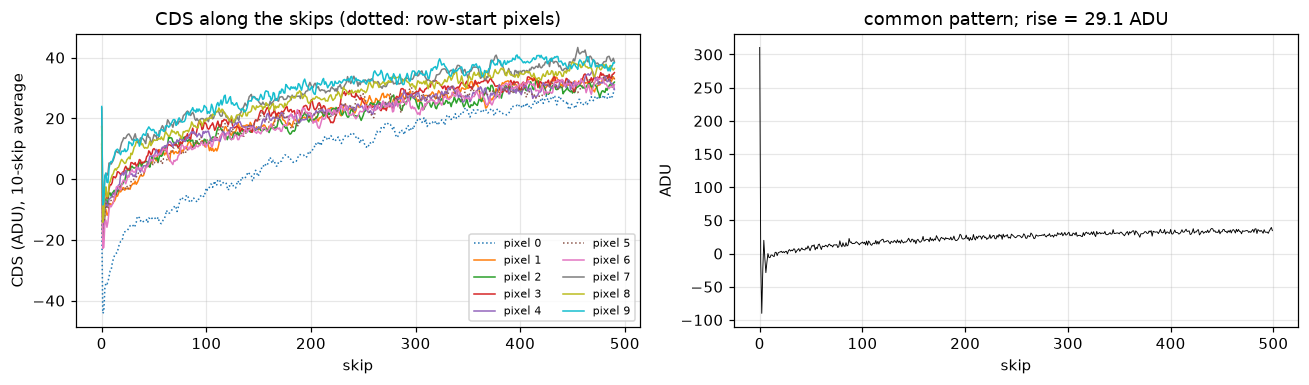
\includegraphics[width=1.0\textwidth,height=0.78\textheight,keepaspectratio]{level_common_pattern.png}
\caption{Left: CDS of every pixel along its 500 skips (10-skip average; dotted: row-start pixels). Right: the common pattern (median of the usable pixels), which rises by about 29 ADU along the skips. Example trace: module 101, channel 0, 2026-10-08, first repeat.}
\label{fig:level_common_pattern}
\end{figure}

\begin{figure}[htbp]
\centering
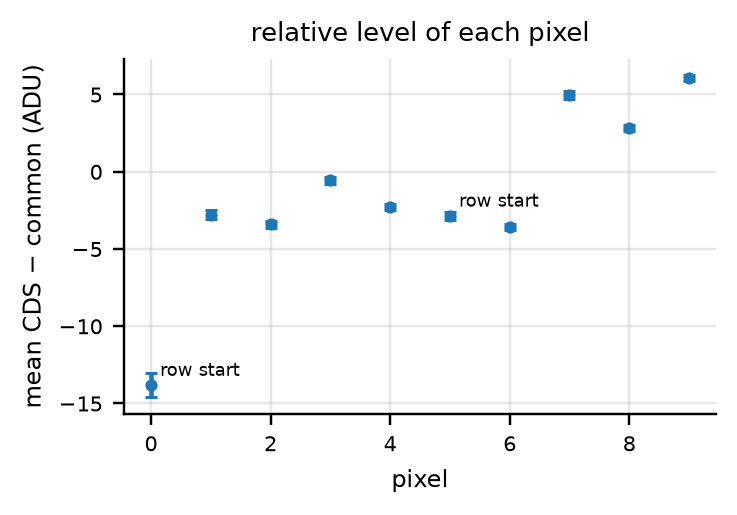
\includegraphics[width=0.5\textwidth,height=0.78\textheight,keepaspectratio]{level_pixel_levels.png}
\caption{Relative CDS level of each pixel (mean CDS minus the common pattern) with its $\pm$1$\sigma$ uncertainty from 10-skip blocks (about $\pm$0.2 ADU). Pixel 0 is a row-start pixel. Example trace: module 101, channel 0, 2026-10-08, first repeat.}
\label{fig:level_pixel_levels}
\end{figure}

\begin{figure}[htbp]
\centering
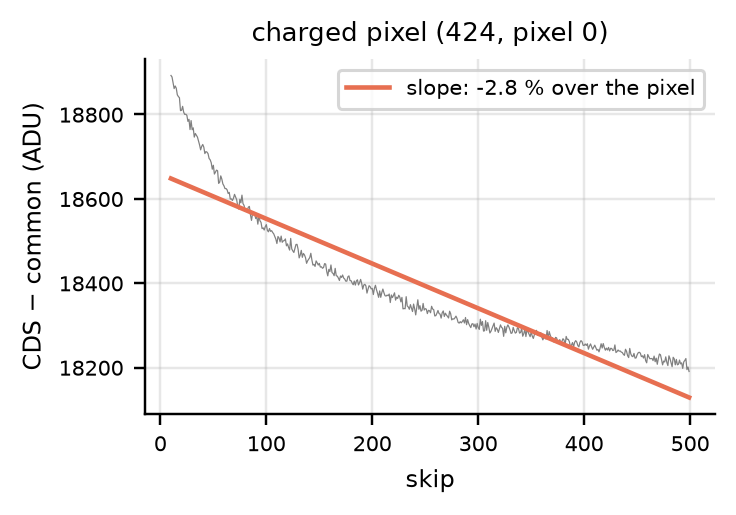
\includegraphics[width=0.5\textwidth,height=0.78\textheight,keepaspectratio]{level_charge_loss.png}
\caption{The charged pixel of the fourth channel-0 repeat (about 18,400 ADU): CDS minus the common pattern along its skips, with a straight-line fit ($-$2.8 \% over the pixel).}
\label{fig:level_charge_loss}
\end{figure}

\clearpage

\section{Advanced features: noise character}
These describe how the noise behaves (correlation, averaging, spectrum, window length, settling, coupling), not only its size. The 2026-10-21 additions (tier 1 and 2, after the original 15) add the null CDS (a CDS between the two halves of the pedestal window, where no charge moves), a jump-robust sigma, the 1/f and Lorentzian corners, drift-insensitive Allan variants, the waveform-mode noise budget and several noise-shape statistics.

\begin{longtable}{>{\raggedright\arraybackslash}p{0.235\textwidth}>{\raggedright\arraybackslash}p{0.075\textwidth}>{\raggedright\arraybackslash}p{0.335\textwidth}>{\raggedright\arraybackslash}p{0.15\textwidth}>{\raggedright\arraybackslash}p{0.07\textwidth}}
\toprule Feature & Unit & What is computed & Possible link & Tier \\ \midrule \endhead
\bottomrule \endfoot
\texttt{noise: CDS autocorrelation at lag 1} &  & Autocorrelation of the detrended CDS (skips 10-499) at lag 1. & how the noise averages down & 0/A2 \\
\texttt{noise: Allan deviation n=50 (ADU)} & ADU & Allan deviation (scatter between consecutive 50-skip means / $\surd$2) of the detrended CDS. & noise after averaging; $\sigma$e-like & 0/A2 P \\
\texttt{noise: Allan slope n=10-100} &  & Log-log slope of the Allan deviation between n = 10 and n = 100 (white noise: $-$0.5). & colour of the noise at large n & 0/C \\
\texttt{noise: CDS power \textless{}1 kHz / \textgreater{}10 kHz} &  & Ratio of the mean spectral density of the detrended CDS sequence (sampled at the skip rate) in its lowest 6.5 \% to that in its top 35 \% (below 1 kHz and above 10 kHz at the usual skip rate of 30.7 kHz). & 1/f vs anticorrelated noise & 0/A2 \\
\texttt{noise: reset-level scatter (ADU)} & ADU & Skip-to-skip standard deviation of each cycle's pedestal-window level after removing the slow droop (polynomial across skips at each sample position). Each reset sets a new random level; the CDS cancels it. & sense node (kTC) and reset gate; related to the gain & 0/B P \\
\texttt{noise: within-cycle power 0.1-0.3 MHz} & fraction & Fraction of the noise power above 0.1 MHz that lies in 0.1-0.3 MHz, from the pedestal-window start to the signal-window end (no reset inside), each cycle's own mean removed. & which part of the chain makes the noise the CDS keeps & 0/A1 \\
\texttt{noise: within-cycle power 0.3-1 MHz} & fraction & Same, 0.3-1 MHz. &  & 0/A1 \\
\texttt{noise: within-cycle power 1-3 MHz} & fraction & Same, 1-3 MHz. &  & 0/A1 \\
\texttt{noise: within-cycle power 3-7.5 MHz} & fraction & Same, 3-7.5 MHz. &  & 0/A1 \\
\texttt{noise: window-length ratio 75/150} &  & CDS recomputed from the raw samples with half-length windows at the start of the real windows; ratio of its detrended noise to that with the full windows (75/150 samples for the usual windows; white noise: 1.41). & how the noise behaves within the integration; delayInt & 0/A2 \\
\texttt{noise: late/early window ratio} &  & Noise of half-length windows ending at the end of the real windows divided by that of half-length windows starting at their start. & settling at the window start & 0/C \\
\texttt{noise: pedestal-window settling (ADU)} & ADU & Mean waveform inside the pedestal window (window mean removed): last 10 samples minus first 10. & window not flat: timing sensitivity & 0/A1 \\
\texttt{noise: signal-window settling (ADU)} & ADU & Same for the signal window. & signal still settling after the SW clock; SW/OG delays & 0/B \\
\texttt{noise: baseline coupling (1e-3)} & $\times$10$^{-3}$ & Slope of the CDS against the skip's baseline level over skips 10-499 of a pixel (the baseline droops by thousands of ADU). & common-mode rejection of the output stage; VDD, VDRAIN, VR & 0/C \\
\texttt{noise: noise trend along skips (ADU/100 skips)} & ADU/\allowbreak{}100 skips & Slope of the standard deviation of 50-skip blocks of the detrended CDS along the pixel. & noise depending on the amplifier operating point & 0/C \\
\texttt{noise: null-CDS noise (ADU)} & ADU & Std over skips of mean(first half) - mean(second half) of the pedestal window of the residual cycles (\#15). & noise without a charge transfer (white: about sqrt(2) x the CDS noise) & 1/A2 P \\
\texttt{noise: jump-robust CDS sigma (ADU)} & ADU & sqrt(MedRV / N) of the detrended CDS (Andersen-Dobrev-Schaumburg median realized variance) (\#25). & continuous noise without jumps & 1/B P \\
\texttt{noise: 1/f corner frequency (kHz)} & kHz & f\_c = (A/W)\textasciicircum{}(1/gamma) of S(f) = W + A f\textasciicircum{}-gamma fitted (in log space) to noise: CDS spectrum, log frequency, clipped to [half the lowest, twice the highest] frequency of the band (\#36). & where 1/f noise takes over from white noise & 1/C \\
\texttt{noise: 1/f exponent} &  & gamma of that fit (\#36). & type of the low-frequency noise & 1/C \\
\texttt{noise: Hadamard deviation n=50 (ADU)} & ADU & Hadamard deviation (third difference of disjoint n-skip means / sqrt 6) of the CDS with only the common pixel pattern removed, not detrended (\#38). & averaging noise, insensitive to linear drift and without the polynomial bias of the detrended Allan & 1/A2 \\
\texttt{noise: CDS variance share of the 3 largest waveform modes} &  & PCA of the residual skip cycles; the fraction of the CDS variance carried by the 3 modes with the most waveform variance (exploratory report, idea 1). & do the big clock / reset fluctuations reach the CDS? (pilot: no) & 1/C \\
\texttt{noise: waveform modes for 90 \% of the CDS variance} &  & Number of modes (by waveform variance) needed to carry 90 \% of the CDS variance. & how concentrated the CDS noise is & 1/A1 \\
\texttt{noise: null-CDS autocorrelation at lag 1} &  & Lag-1 autocorrelation of the null CDS along the skips (\#17). & slow change of the in-window slope & 2/B \\
\texttt{noise: volatility clustering (Ljung-Box of e\textasciicircum{}2, 10 lags)} &  & Ljung-Box Q of the squared detrended CDS, 10 lags (\#30). & bursty noise regimes (ARCH) & 2/C \\
\texttt{noise: Lorentzian corner (kHz)} & kHz & f\_L of S(f) = W + B / (1 + (f/f\_L)\textasciicircum{}2) fitted to the log-frequency CDS spectrum (\#37). & RTS rate (Machlup) & 2/C \\
\texttt{noise: structure-function excess at 9 blocks (ADU)} & ADU & sqrt(max(D(9)\textasciicircum{}2 - D(1)\textasciicircum{}2, 0)) of that curve (\#24). & slow in-window noise (RTS with long dwell) & 2/A1 \\
\texttt{noise: lag-1 autocorrelation of 10-skip means} &  & Lag-1 autocorrelation of disjoint 10-skip means of the detrended CDS (\#40). & noise type at the 10-skip scale & 2/B \\
\texttt{noise: DFA exponent} &  & Detrended-fluctuation-analysis exponent of the detrended CDS (scales 4-48 skips). & long-range correlation (cardiology); mostly new information (R\textasciicircum{}2 0.15) & 2/C \\
\texttt{noise: CDS spectral slope} &  & Slope of log power against log frequency of the detrended CDS. & noise colour; new information (R\textasciicircum{}2 0.40) & 2/A2 \\
\texttt{noise: CDS spectral centroid} &  & Mean frequency (fraction of the Nyquist) of the CDS power spectrum. & separates amplifiers strongly (F 63) & 2/A2 \\
\texttt{noise: sample entropy} &  & Sample entropy (m = 2, r = 0.2 sd) of the detrended CDS. & regularity (nonlinear dynamics) & 2/A2 \\
\texttt{noise: permutation entropy (m=4)} &  & Normalized permutation entropy, order 4, of the detrended CDS. & ordinal structure & 2/A2 \\
\texttt{noise: red-noise beta (50 skips)} &  & Std of 50-skip bin means / (std / sqrt 50) of the detrended CDS (astronomy beta factor). & excess noise at the 50-skip scale & 2/B \\
\texttt{noise: baseline-CDS residual correlation} &  & Correlation of the detrended per-skip pedestal level with the detrended CDS (\#42). & common supply or reset disturbance & 2/C \\
\end{longtable}

\begin{figure}[htbp]
\centering
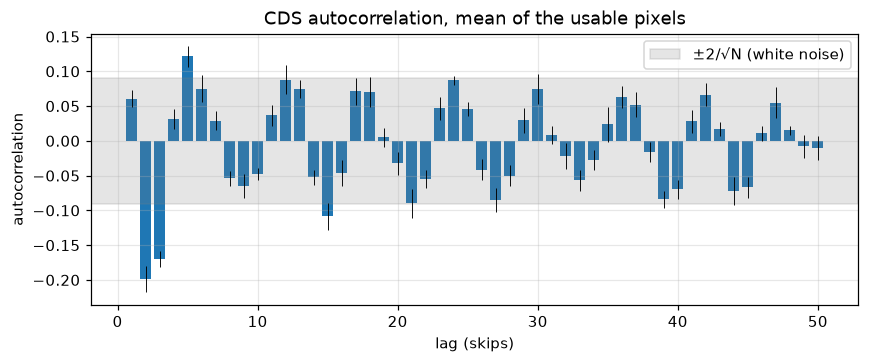
\includegraphics[width=0.5\textwidth,height=0.78\textheight,keepaspectratio]{noise_autocorrelation.png}
\caption{Autocorrelation of the detrended CDS, lags 1--50 (mean of the usable pixels); grey band: $\pm$2/$\surd$N expected for white noise. Lags 2 and 3 are about $-$0.2. Example trace: module 101, channel 0, 2026-10-08, first repeat.}
\label{fig:noise_autocorrelation}
\end{figure}

\begin{figure}[htbp]
\centering
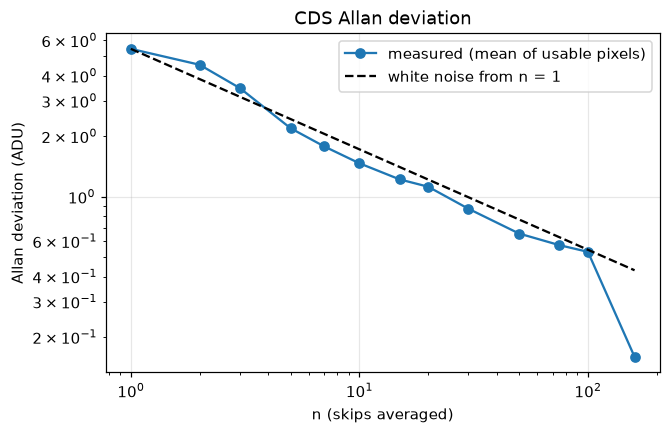
\includegraphics[width=0.5\textwidth,height=0.78\textheight,keepaspectratio]{noise_allan.png}
\caption{Allan deviation of the detrended CDS (mean of the usable pixels); dashed: white noise scaled from n = 1. Example trace: module 101, channel 0, 2026-10-08, first repeat.}
\label{fig:noise_allan}
\end{figure}

\begin{figure}[htbp]
\centering
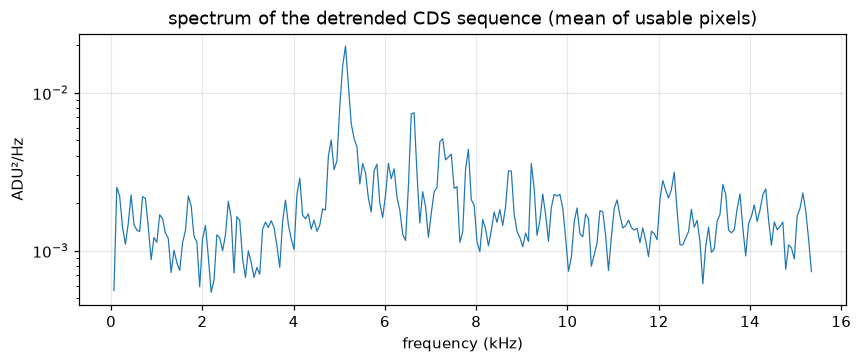
\includegraphics[width=0.5\textwidth,height=0.78\textheight,keepaspectratio]{noise_cds_spectrum.png}
\caption{Spectral density of the detrended CDS sequence (sampled at the skip rate, 0--15 kHz); note the peak near 5 kHz. Example trace: module 101, channel 0, 2026-10-08, first repeat.}
\label{fig:noise_cds_spectrum}
\end{figure}

\begin{figure}[htbp]
\centering
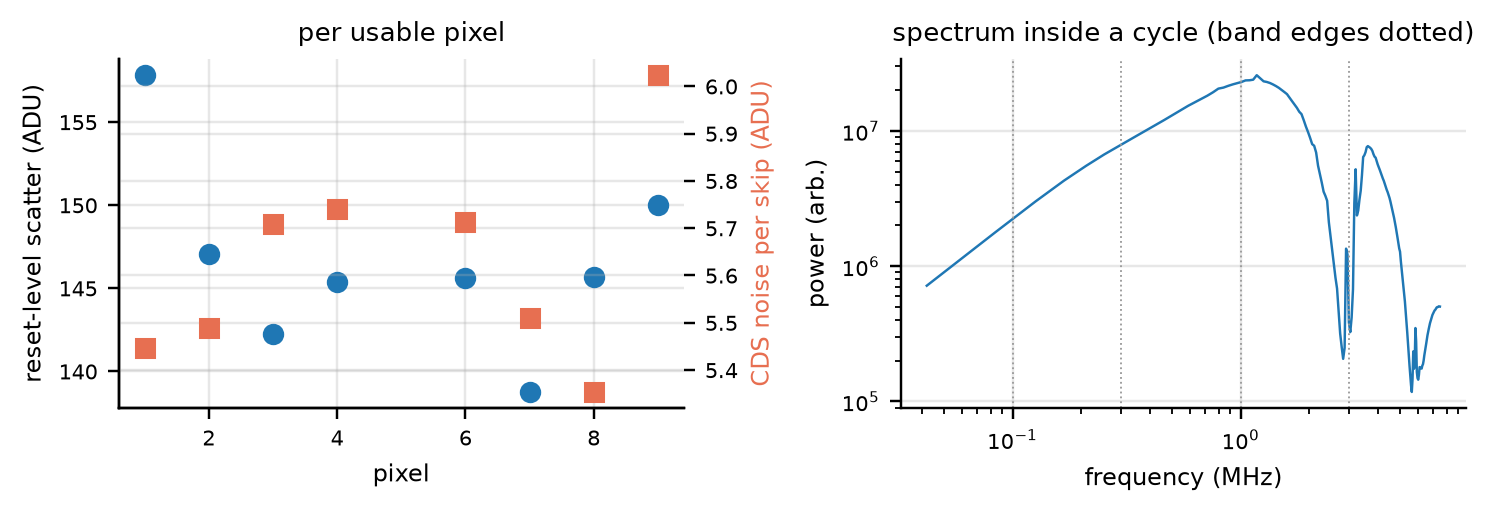
\includegraphics[width=1.0\textwidth,height=0.78\textheight,keepaspectratio]{noise_reset_and_bands.png}
\caption{Left: reset-level scatter (about 146 ADU) and CDS noise per skip (about 5.6 ADU) for each usable pixel. Right: noise spectrum inside a cycle (pedestal-window start to signal-window end, each cycle's own mean removed). Example trace: module 101, channel 0, 2026-10-08, first repeat.}
\label{fig:noise_reset_and_bands}
\end{figure}

\begin{figure}[htbp]
\centering
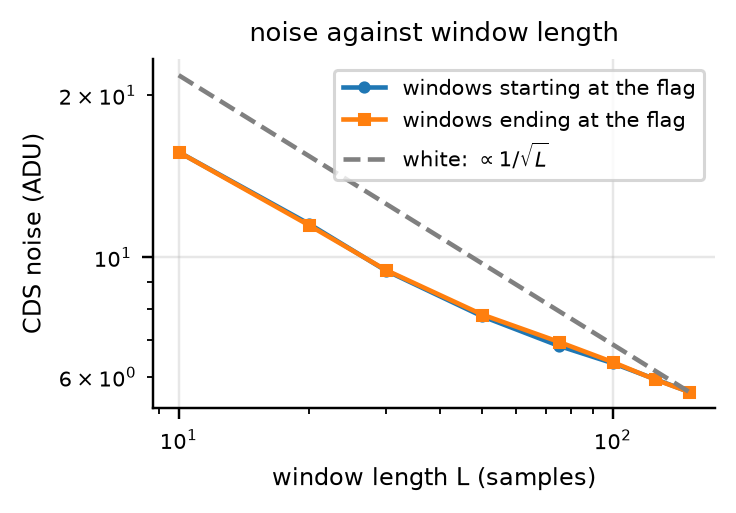
\includegraphics[width=0.5\textwidth,height=0.78\textheight,keepaspectratio]{noise_window_length.png}
\caption{CDS noise per skip recomputed with shorter windows (circles: windows starting at the flag; squares: windows ending at the flag), against 1/$\surd$L white noise (dashed). Example trace: module 101, channel 0, 2026-10-08, first repeat.}
\label{fig:noise_window_length}
\end{figure}

\begin{figure}[htbp]
\centering
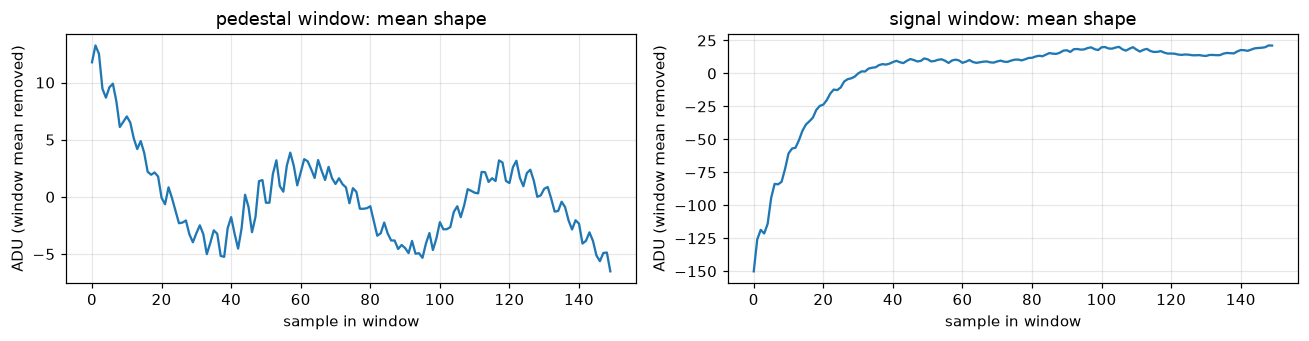
\includegraphics[width=1.0\textwidth,height=0.78\textheight,keepaspectratio]{noise_window_settling.png}
\caption{Mean waveform inside the pedestal window (left) and the signal window (right), window mean removed. The signal window starts about 150 ADU low and settles within about 30 samples (2 $\mu$s). Example trace: module 101, channel 0, 2026-10-08, first repeat.}
\label{fig:noise_window_settling}
\end{figure}

\begin{figure}[htbp]
\centering
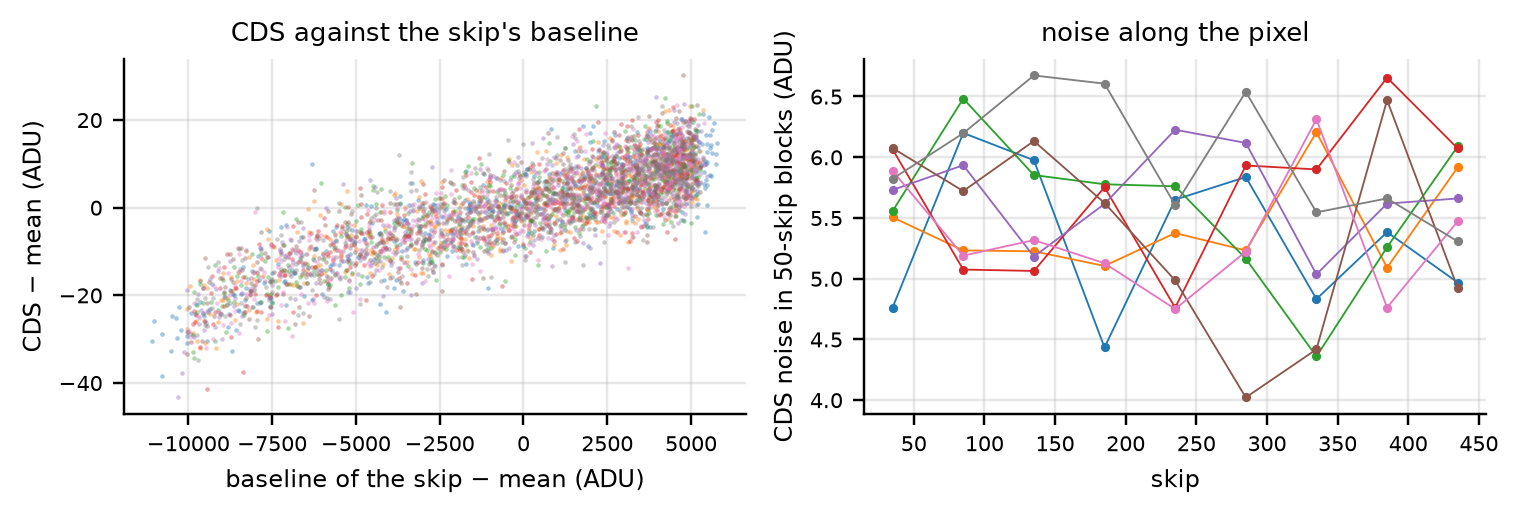
\includegraphics[width=1.0\textwidth,height=0.78\textheight,keepaspectratio]{noise_baseline_coupling.png}
\caption{Left: CDS against the baseline level of each skip (usable pixels); the slope is the baseline coupling (about 2.1$\times$10$^{-3}$). Right: CDS noise in 50-skip blocks along the pixel. Example trace: module 101, channel 0, 2026-10-08, first repeat.}
\label{fig:noise_baseline_coupling}
\end{figure}

\clearpage

\section{Advanced features: discrete and transient noise}
Steps, heavy tails, interference lines and ADC code non-uniformity. The 2026-10-21 additions detect telegraph steps inside single windows, split the CDS variance into a smooth part and jumps, give calibrated jump counts, and find pickup lines with a stated false-alarm rate (multitaper F-test).

\begin{longtable}{>{\raggedright\arraybackslash}p{0.235\textwidth}>{\raggedright\arraybackslash}p{0.075\textwidth}>{\raggedright\arraybackslash}p{0.335\textwidth}>{\raggedright\arraybackslash}p{0.15\textwidth}>{\raggedright\arraybackslash}p{0.07\textwidth}}
\toprule Feature & Unit & What is computed & Possible link & Tier \\ \midrule \endhead
\bottomrule \endfoot
\texttt{discrete: largest baseline step (t)} &  & Largest difference between the 20-skip means before and after a skip of the detrended per-skip baseline, in units of its standard error. & telegraph noise in the output transistor & 0/B \\
\texttt{discrete: largest CDS step (t)} &  & Same for the detrended CDS (chance level for 490 skips: about 4). & telegraph noise & 0/C \\
\texttt{discrete: CDS excess kurtosis} &  & Excess kurtosis of the detrended CDS. & heavy tails: glitches, bursts & 0/A2 \\
\texttt{discrete: CDS outlier fraction} &  & Fraction of skips more than 5 robust $\sigma$ from the median of the detrended CDS. & glitches, bursts, charge arriving during readout & 0/A2 \\
\texttt{discrete: CDS spectrum lines} & count & Number of peaks more than 5$\times$ above the local median in the CDS spectrum. & periodic pickup & 0/A2 \\
\texttt{discrete: within-cycle spectrum lines} & count & Same in the within-cycle spectrum. & periodic pickup & 0/C \\
\texttt{discrete: ADC low-bit chi2/dof} &  & $\chi$$^{2}$ per degree of freedom of the histogram of (sample value mod 64) inside the pedestal windows against a flat distribution. & ADC differential non-linearity (channel health) & 0/C \\
\texttt{discrete: null-CDS kurtosis} &  & Excess kurtosis of the null CDS (\#16). & non-Gaussian noise in the output stage, separate from the transfer (RTS) & 1/A2 \\
\texttt{discrete: in-window step rate (\%)} & \% & Percentage of windows (pedestal and signal, skips from the noise start) whose best single step in 10-sample block means has t \textgreater{} 6 (\#18). & random-telegraph switching rate x detection efficiency & 1/A2 \\
\texttt{discrete: in-window step amplitude (ADU)} & ADU & Median |step| of the detected in-window steps (\#19). & RTS amplitude x gain (trap size) & 1/C \\
\texttt{discrete: jump share of CDS variance} &  & 1 - MedRV / RV of the detrended CDS (\#26). & fraction of the CDS variance in jumps & 1/A2 \\
\texttt{discrete: line count (F-test, p\textless{}0.001)} &  & Frequencies where the multitaper Thomson F statistic (NW = 3, K = 5) of the detrended CDS exceeds F(2, 2K-2) at p = 0.001 in at least half of the usable pixels (\#32). & pickup lines with a stated false-alarm rate & 1/C \\
\texttt{discrete: strongest line frequency (kHz)} & kHz & Frequency of the largest median F (\#33). & identifies the pickup source & 1/C \\
\texttt{discrete: strongest line amplitude (ADU)} & ADU & Median over pixels of the multitaper line amplitude 2|mu| at that frequency (\#33). & pickup size & 1/A2 \\
\texttt{discrete: line phase coherence, pixel clock} &  & |mean\_p exp(i phi\_p)| with phi\_p the line phase referred to each pixel's own first skip (\#34). & 1 = the line is made by the readout sequence (clock-locked) & 1/C \\
\texttt{discrete: line phase coherence, absolute time} &  & The same with the phase referred to absolute time in the trace. & 1 = an external source running continuously & 1/C \\
\texttt{discrete: jump count (Lee-Mykland, 1 \%)} &  & Number of skips whose |e\_k| / local bipower sigma (20 skips) exceeds the 1 \% Gumbel critical value of Lee \& Mykland, with c = sqrt(2/pi) (\#27). With a 20-skip window pure Gaussian noise still gives $\sim$0.26 per series: a relative count. & jump count (relative) & 2/A2 \\
\texttt{discrete: STA/LTA maximum} &  & max\_k mean(e\textasciicircum{}2, k..k+4) / mean(e\textasciicircum{}2, k-50..k-1) of the detrended CDS (\#28). & localized bursts (seismology trigger) & 2/A2 \\
\texttt{discrete: crest factor} &  & max |e| / std(e) of the detrended CDS (\#29). & largest excursion & 2/A2 \\
\texttt{discrete: whitened CDS kurtosis} &  & Excess kurtosis of the detrended CDS after dividing its FFT by the square root of its smoothed spectrum (\#31). & non-Gaussianity without the colour of 1/f noise and pickup & 2/A2 \\
\texttt{discrete: max within-window spectral kurtosis} &  & max over f of the spectral kurtosis of the pedestal windows of the residual cycles (\#45). & frequency band of impulsive noise & 2/B \\
\texttt{discrete: line frequency, whole trace (kHz)} & kHz & Peak of the Lomb-Scargle periodogram of the detrended CDS of all usable pixels in absolute time, 0.2-15 kHz (\#35). & fine frequency resolution across the trace & 2/C \\
\end{longtable}

\begin{figure}[htbp]
\centering
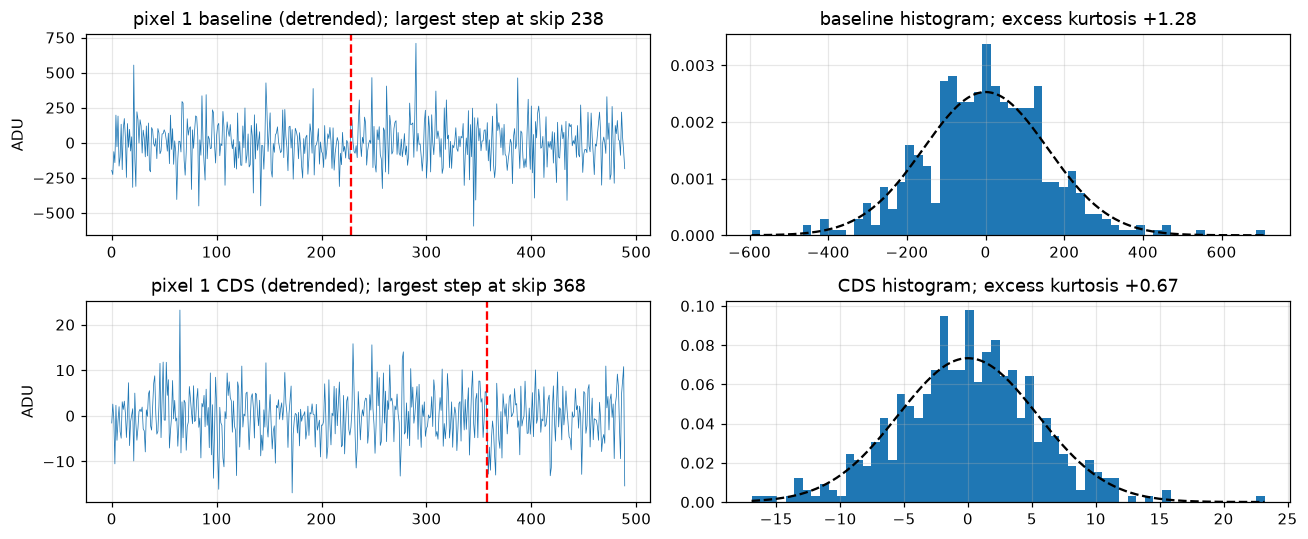
\includegraphics[width=1.0\textwidth,height=0.78\textheight,keepaspectratio]{discrete_steps.png}
\caption{Detrended baseline (top) and CDS (bottom) of one pixel, with the position of the largest step (dashed), and their histograms with a Gaussian of the same variance. No telegraph noise is seen. Example trace: module 101, channel 0, 2026-10-08, first repeat.}
\label{fig:discrete_steps}
\end{figure}

\begin{figure}[htbp]
\centering
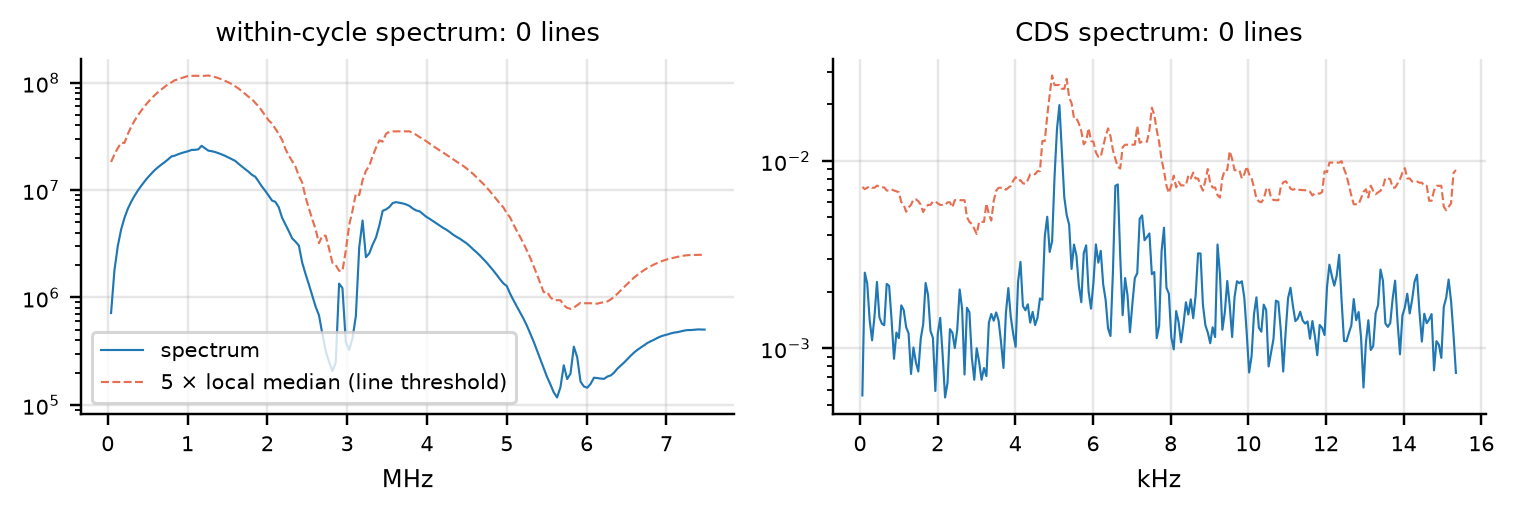
\includegraphics[width=1.0\textwidth,height=0.78\textheight,keepaspectratio]{discrete_lines.png}
\caption{Line search in the within-cycle spectrum (left, MHz) and the CDS spectrum (right, kHz); no peak exceeds 5 times the local median in this trace. Example trace: module 101, channel 0, 2026-10-08, first repeat.}
\label{fig:discrete_lines}
\end{figure}

\begin{figure}[htbp]
\centering
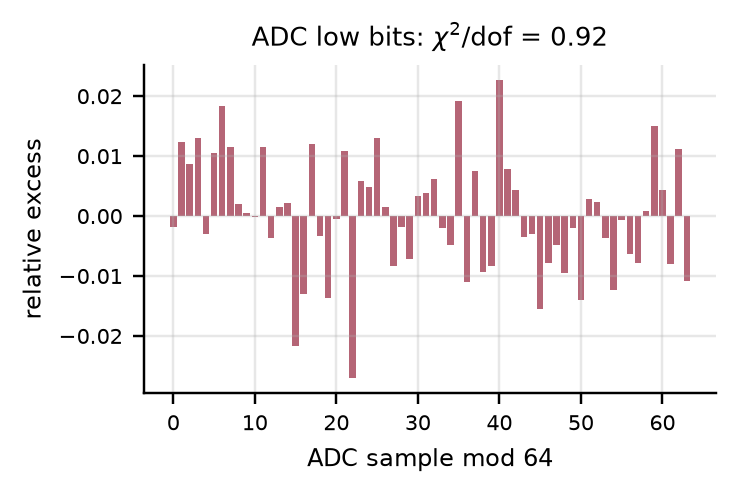
\includegraphics[width=0.5\textwidth,height=0.78\textheight,keepaspectratio]{discrete_adc_codes.png}
\caption{Relative excess of each value of (ADC sample mod 64) inside the pedestal windows; $\chi$$^{2}$ = 58 for 63 degrees of freedom (flat). Example trace: module 101, channel 0, 2026-10-08, first repeat.}
\label{fig:discrete_adc_codes}
\end{figure}

\clearpage

\section{Advanced features: edges}
From the reset pulse and the summing-well dip: timing, sub-sample shape, recovery, coupling per volt, and the skip-to-skip variation along the cycle. Added 2026-10-21: the sharp dip about 120--130 ns before the reset pulse, measured on the equivalent-time pulse.

\begin{longtable}{>{\raggedright\arraybackslash}p{0.235\textwidth}>{\raggedright\arraybackslash}p{0.075\textwidth}>{\raggedright\arraybackslash}p{0.335\textwidth}>{\raggedright\arraybackslash}p{0.15\textwidth}>{\raggedright\arraybackslash}p{0.07\textwidth}}
\toprule Feature & Unit & What is computed & Possible link & Tier \\ \midrule \endhead
\bottomrule \endfoot
\texttt{edge: jitter (ns)} & ns & Scatter of the reset-edge times (half-height crossing, linear interpolation) around a straight line in skip number. & timing jitter; matters where windows sit on slopes & 0/A1 \\
\texttt{edge: period offset (1e-3 samples)} & $\times$10$^{-3}$ samples & Slope of that line minus 488.7. Small differences between amplifiers come from the edge-time estimate drifting with the baseline droop, not from the clock. & edge-shape change along the pixel & 0/A1 \\
\texttt{edge: rise time (ns)} & ns & 10-90 \% rise time of the reset pulse rebuilt by equivalent-time sampling (samples placed at their exact time relative to the edge line, 0.1-sample bins; crossings interpolated). & video-chain bandwidth & 0/A1 \\
\texttt{edge: recovery tau1 (us)} & $\mu$s & Faster time constant of two exponentials fitted to the equivalent-time waveform after the pulse peak. & amplifier response & 0/A2 \\
\texttt{edge: recovery tau2 (us)} & $\mu$s & Slower time constant of that fit. & amplifier response & 0/A1 \\
\texttt{edge: recovery amplitude ratio} &  & Amplitude of the fast exponential divided by that of the slow one. & amplifier response & 0/A1 \\
\texttt{edge: ringing frequency (MHz)} & MHz & Strongest frequency in the residual of that fit over the first 25 samples after the peak (zero-padded spectrum, peak refined by a parabola). & amplifier stability/bandwidth & 0/A1 \\
\texttt{edge: ringing rms (ADU)} & ADU & RMS of the residual of that fit over the first 25 samples after the peak. & amplifier stability & 0/A1 \\
\texttt{edge: dip per volt SW (ADU/V)} & ADU/\allowbreak{}V & Dip height divided by the summing-well swing SW\_1\_H $-$ SW\_1\_L (from the .meta; NaN without it). Assumes the channel uses SW\_1. & coupling $\times$ amplification (gain-related) & 0/B P \\
\texttt{edge: pulse per volt RG (ADU/V)} & ADU/\allowbreak{}V & Reset-pulse height above the signal level divided by RG\_1\_H $-$ RG\_1\_L. & coupling $\times$ amplification (gain-related) & 0/A1 P \\
\texttt{edge: pulse/dip ratio} &  & Reset-pulse height divided by dip height; the common amplification cancels. & relative coupling & 0/B \\
\texttt{edge: cycle variation in signal window (ADU)} & ADU & Median, inside the signal window, of the standard deviation across skips at each sample position (each skip's pedestal level subtracted). & noise that enters the CDS & 0/B \\
\texttt{edge: cycle variation at dip (ADU)} & ADU & Maximum of that profile around the dip. & timing (phase walk, jitter) $\times$ edge steepness & 0/A1 \\
\texttt{edge: cycle variation at reset (ADU)} & ADU & Maximum of that profile around the reset pulse. & timing $\times$ edge steepness & 0/A2 \\
\texttt{edge: cycle variation after reset (ADU)} & ADU & Median of that profile after the reset (sample 420 to the end of the cycle). & reset level scatter seen within the cycle & 0/B \\
\texttt{edge: pre-pulse dip depth (ADU)} & ADU & Minimum of the equivalent-time pulse between 6 and 0 samples before the edge, minus its mean 15-8 samples before (a sharp dip $\sim$120-130 ns before the pulse, $\sim$1.5 samples wide, so single cycles show it as one low sample). & feedthrough of a clock edge just before the pulse (SW/RG/OG, not yet identified); pilot: amplifier-specific, repeat share 0.001 & 1/A1 \\
\texttt{edge: pre-pulse dip / pulse height} &  & That depth divided by the height of the equivalent-time pulse above the same baseline. & coupling of that edge relative to the pulse; the common amplification cancels & 1/B \\
\end{longtable}

\begin{figure}[htbp]
\centering
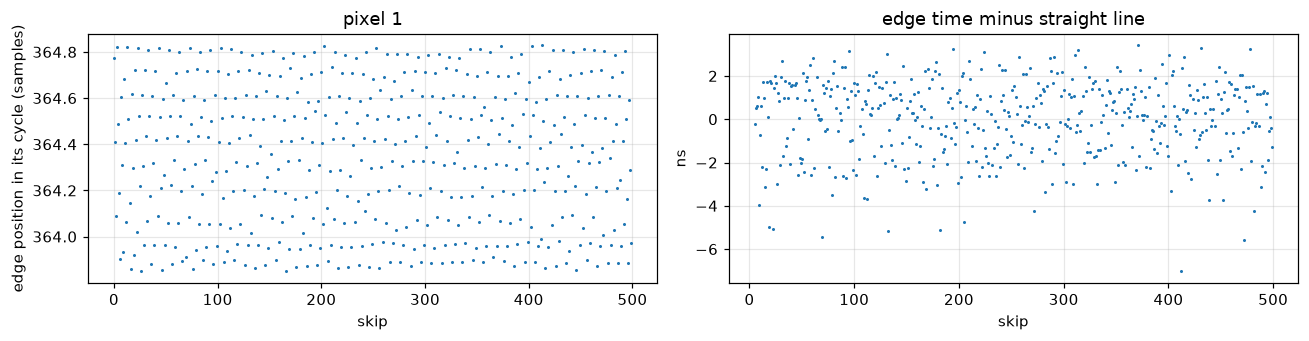
\includegraphics[width=1.0\textwidth,height=0.78\textheight,keepaspectratio]{edge_jitter.png}
\caption{Left: position of the reset edge inside its own cycle; it saws by a third of a sample because the cycle is 488.7 samples long but starts on whole samples. Right: edge time minus the straight-line fit against the skip number (jitter about 1.7 ns rms). Example trace: module 101, channel 0, 2026-10-08, first repeat.}
\label{fig:edge_jitter}
\end{figure}

\begin{figure}[htbp]
\centering
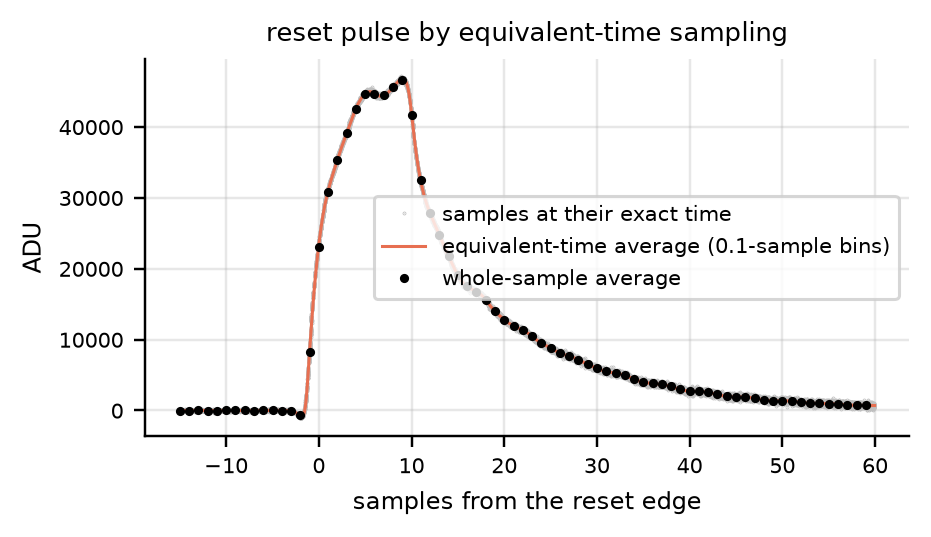
\includegraphics[width=0.62\textwidth,height=0.78\textheight,keepaspectratio]{edge_equivalent_time.png}
\caption{The reset pulse rebuilt by equivalent-time sampling (red, 0.1-sample bins) compared with the plain average of whole samples (dots); grey: individual samples at their exact time. Example trace: module 101, channel 0, 2026-10-08, first repeat.}
\label{fig:edge_equivalent_time}
\end{figure}

\begin{figure}[htbp]
\centering
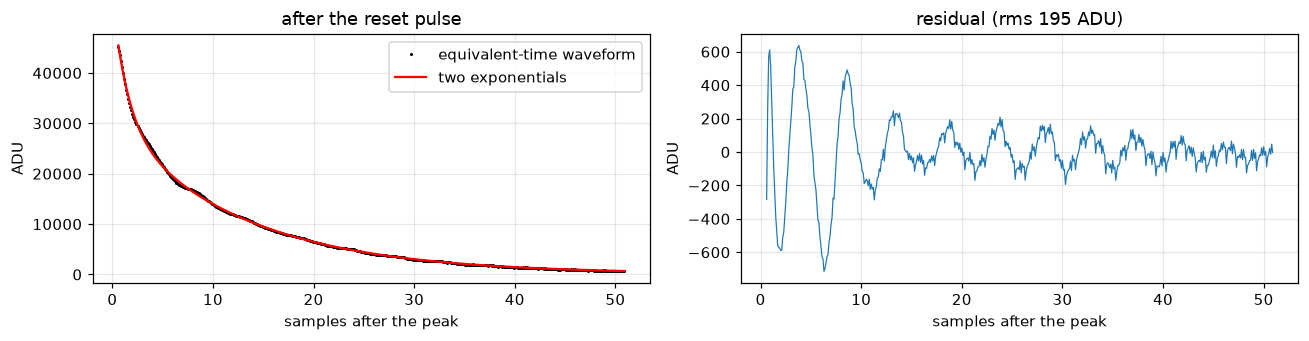
\includegraphics[width=1.0\textwidth,height=0.78\textheight,keepaspectratio]{edge_recovery_ringing.png}
\caption{Left: equivalent-time waveform after the pulse peak with a two-exponential fit. Right: the residual, a decaying oscillation at about 3 MHz (ringing). Example trace: module 101, channel 0, 2026-10-08, first repeat.}
\label{fig:edge_recovery_ringing}
\end{figure}

\begin{figure}[htbp]
\centering
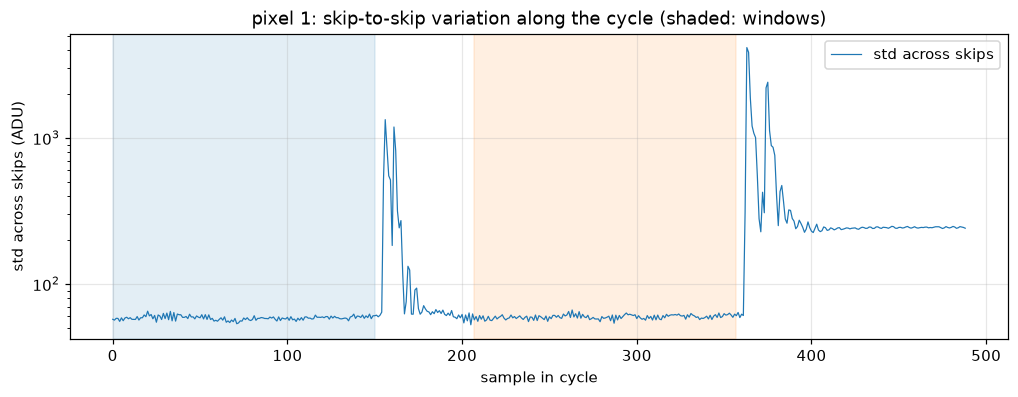
\includegraphics[width=1.0\textwidth,height=0.78\textheight,keepaspectratio]{edge_cycle_variation.png}
\caption{Standard deviation across skips at every position of the cycle (each skip's pedestal level removed); shaded: pedestal and signal windows. Small and flat inside the windows, large at the dip and the reset pulse, a few hundred ADU after the reset. Example trace: module 101, channel 0, 2026-10-08, first repeat.}
\label{fig:edge_cycle_variation}
\end{figure}

\clearpage

\section{Advanced features: slow structure}
Row-start recovery, drift across the trace, horizontal-transfer amplitude and principal components.

\begin{longtable}{>{\raggedright\arraybackslash}p{0.235\textwidth}>{\raggedright\arraybackslash}p{0.075\textwidth}>{\raggedright\arraybackslash}p{0.335\textwidth}>{\raggedright\arraybackslash}p{0.15\textwidth}>{\raggedright\arraybackslash}p{0.07\textwidth}}
\toprule Feature & Unit & What is computed & Possible link & Tier \\ \midrule \endhead
\bottomrule \endfoot
\texttt{slow: row-start recovery time (skips)} & skips & Time constant of an exponential fitted to the baseline of the second row-start pixel minus that of the next pixel, skip by skip. & electronics recovering from the vertical clocking & 0/B \\
\texttt{slow: row-start recovery amplitude (ADU)} & ADU & Amplitude of that exponential. & vertical clock coupling & 0/A1 \\
\texttt{slow: drift (ADU/ms)} & ADU/\allowbreak{}ms & Slope of the baseline at the middle skip (250 of 500) of successive usable pixels against time in the trace. & slow drift (thermal, supplies) & 0/C \\
\texttt{slow: H-transfer peak-to-peak (ADU)} & ADU & Peak-to-peak amplitude of a horizontal transfer, mean over transfers and usable pixels. & H-clock coupling & 0/B \\
\texttt{slow: H-transfer first-to-last change (ADU)} & ADU & Peak-to-peak of the last complete transfer minus that of the first. & change along the transfers (charge in the serial register?) & 0/A1 \\
\texttt{slow: PC1 variance fraction} & fraction & Fraction of the skip-to-skip variation (residual cycles of the usable pixels) in the first principal component (in the example trace: the sub-sample phase walk). & structure of the skip-to-skip variation & 0/A2 \\
\texttt{slow: PC2 variance fraction} & fraction & Same, second component (in the example: the level shift set by each reset). &  & 0/B \\
\texttt{slow: PC3 variance fraction} & fraction & Same, third component. &  & 0/B \\
\end{longtable}

\begin{figure}[htbp]
\centering
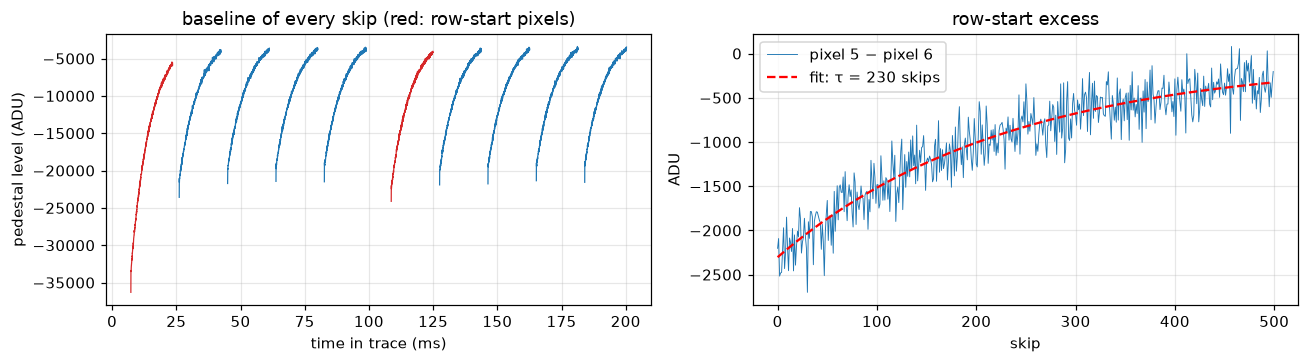
\includegraphics[width=1.0\textwidth,height=0.78\textheight,keepaspectratio]{slow_row_start.png}
\caption{Left: baseline of every skip through the trace (red: row-start pixels). Right: baseline of the second row-start pixel minus that of the next pixel, with an exponential fit (about 230 skips). Example trace: module 101, channel 0, 2026-10-08, first repeat.}
\label{fig:slow_row_start}
\end{figure}

\begin{figure}[htbp]
\centering
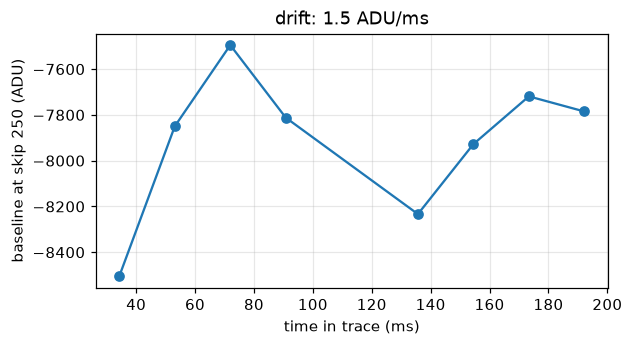
\includegraphics[width=0.5\textwidth,height=0.78\textheight,keepaspectratio]{slow_drift.png}
\caption{Baseline at skip 250 of successive usable pixels against time in the trace; the slope is the drift feature. Example trace: module 101, channel 0, 2026-10-08, first repeat.}
\label{fig:slow_drift}
\end{figure}

\begin{figure}[htbp]
\centering
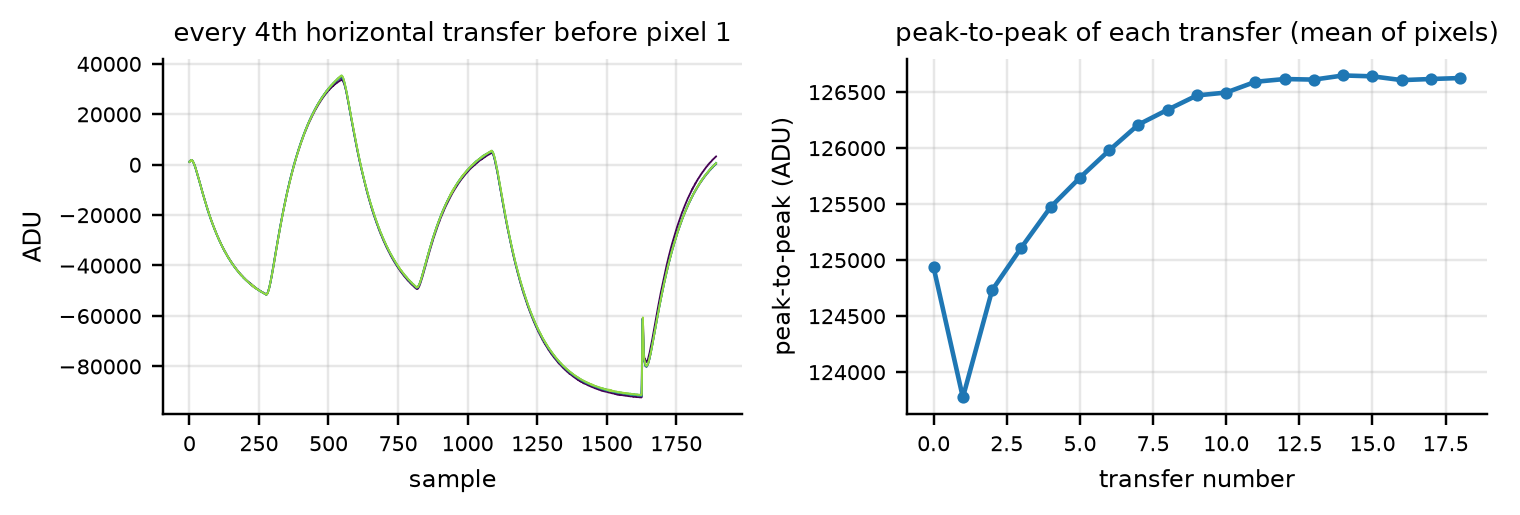
\includegraphics[width=1.0\textwidth,height=0.78\textheight,keepaspectratio]{slow_h_transfers.png}
\caption{Left: every 4th horizontal transfer before a pixel. Right: peak-to-peak amplitude of each transfer (mean of the usable pixels). Example trace: module 101, channel 0, 2026-10-08, first repeat.}
\label{fig:slow_h_transfers}
\end{figure}

\begin{figure}[htbp]
\centering
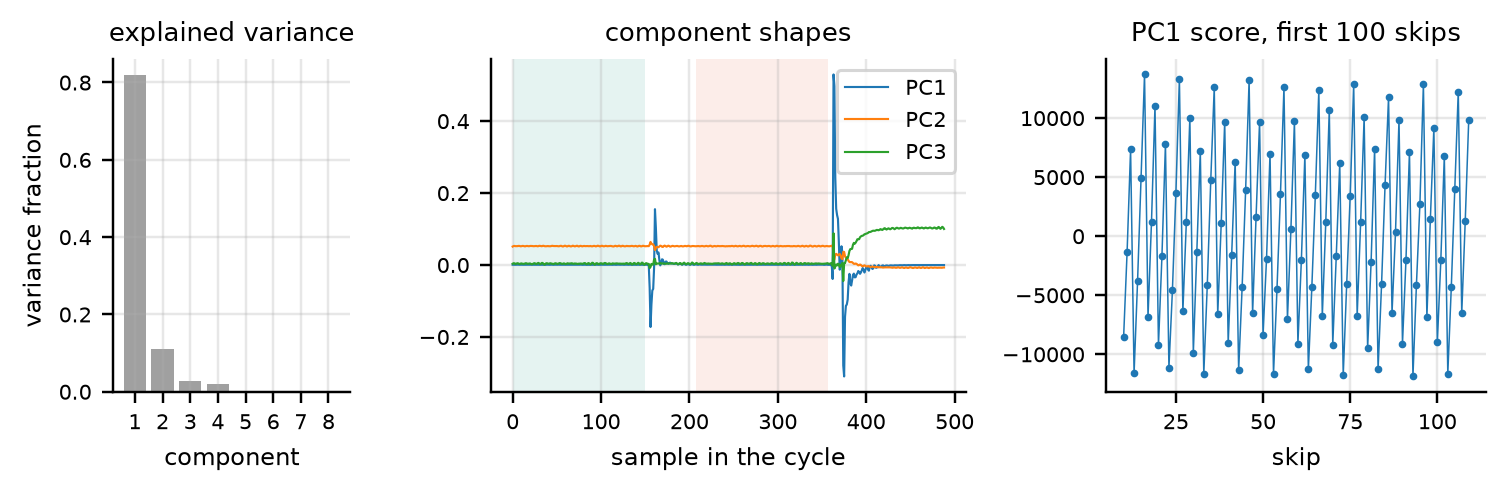
\includegraphics[width=1.0\textwidth,height=0.78\textheight,keepaspectratio]{slow_principal_components.png}
\caption{Principal components of the skip-to-skip variation: explained variance (left), the first three component shapes (centre; shaded: windows) and the PC1 score along the skips (right). PC1 (82 \%) is the sub-sample phase walk at the edges; PC2 is the level shift set by each reset. Example trace: module 101, channel 0, 2026-10-08, first repeat.}
\label{fig:slow_principal_components}
\end{figure}

\clearpage

\section{Start of the pixel (added 2026-10-21)}
The first skips of every pixel read a decaying baseline: the CDS of skip $k$ is offset by the baseline slope inside the windows times the separation of the window centres (about $-207$ samples), so the first-skip offset is a baseline slope, not charge. Its size follows the horizontal-clock swing (H-clock feedthrough). Computed per usable pixel from its first skips: the slope regression uses skips 0--19, the mean transient skips 0--29; the window slopes are compared with their median over skips 20--59 and the CDS with its median from skip 10 on. Per-pixel features are the median over the usable pixels.

\begin{longtable}{>{\raggedright\arraybackslash}p{0.235\textwidth}>{\raggedright\arraybackslash}p{0.075\textwidth}>{\raggedright\arraybackslash}p{0.335\textwidth}>{\raggedright\arraybackslash}p{0.15\textwidth}>{\raggedright\arraybackslash}p{0.07\textwidth}}
\toprule Feature & Unit & What is computed & Possible link & Tier \\ \midrule \endhead
\bottomrule \endfoot
\texttt{start: CDS-slope lever arm (samples)} & samples & Slope of the regression of CDS\_k - median(CDS of later skips) on the in-window baseline slope excess Delta\_k - late (Delta = mean of the pedestal- and signal-window slopes; late = median of skips 20-59), skips 0-19, pooled over the usable pixels (\#2). & about -(window-centre separation) if the first-skip pattern is pure baseline slope; a departure means a charge or gain effect & 1/A2 \\
\texttt{start: slope-explained fraction} &  & R\textasciicircum{}2 of that regression (\#3). & how much of the first-skip pattern is baseline slope & 1/A2 \\
\texttt{start: in-cycle slope at skip 0 (ADU/us)} & ADU/\allowbreak{}$\mu$s & Delta\_0 - late, in ADU per microsecond (\#1). & derivative of the start transient & 1/A1 \\
\texttt{start: transient time constant (us)} & $\mu$s & Time constant of A exp(-t/tau) + c fitted to the skip-0 waveform minus the late mean waveform (each skip minus its pedestal mean), on the pedestal and signal windows only (\#4). & recovery of the video chain / output stage after the H-clock burst & 1/C \\
\texttt{start: transient amplitude (ADU)} & ADU & Amplitude A of that fit at the start of the cycle (\#5). & size of the H-clock disturbance & 1/B \\
\texttt{start: first-skip excess per volt H (ADU/V)} & ADU/\allowbreak{}V & skip: first-skip CDS excess divided by the H1\_A clock swing (H1\_A\_H - H1\_A\_L, .meta) (\#6). & H-clock coupling per volt, comparable across settings & 1/A1 \\
\texttt{start: row-start/inner first-skip ratio} &  & Median first-skip excess of the row-start pixels / that of the usable pixels (\#7). & memory of the clocking before the pixel (prescan, vertical transfers) & 2/B \\
\texttt{start: reset jump skip 0 to 1 (ADU)} & ADU & Pedestal mean of skip 1 minus that of skip 0 (\#8). & first reset after the transfers; operating point of the sense node & 2/A2 \\
\texttt{start: mode frequency (kHz)} & kHz & Frequency of the strongest oscillating pole of a matrix-pencil fit (order 4) of the mean transient, skips 0-29 (\#9). & the start ringing in physical units & 2/C \\
\texttt{start: mode damping (us)} & $\mu$s & Damping time of that pole (\#9). &  & 2/C \\
\texttt{start: fast decay (us)} & $\mu$s & Decay time of the non-oscillating pole with the largest amplitude among those decaying within 10 skips (\#9). &  & 2/C \\
\texttt{start: transient amplitude, matched filter (ADU)} & ADU & Projection of each pixel's CDS of skips 0-29 minus its median CDS from skip 10 on, onto the trace's mean transient, times its peak (\#10). & per-pixel transient size with less noise than the first-skip excess & 2/A1 \\
\texttt{start: ringing frequency (kHz)} & kHz & fit: first-skip ringing frequency (cyc/skip) x the skip rate (\#11). & comparable across delayInt settings & 2/C \\
\end{longtable}


\section{Clocking regions (added 2026-10-21)}
From the vertical-transfer block before the second row (its first transfer, which follows the skip region, left out), the horizontal transfers before each pixel, and the block the trace starts in. The trace starts at a random point inside its first vertical block (14--19 of 20 transfers recorded on 2026-10-12), so the slope of that block is stored (tier 2) but not repeatable.

\begin{longtable}{>{\raggedright\arraybackslash}p{0.235\textwidth}>{\raggedright\arraybackslash}p{0.075\textwidth}>{\raggedright\arraybackslash}p{0.335\textwidth}>{\raggedright\arraybackslash}p{0.15\textwidth}>{\raggedright\arraybackslash}p{0.07\textwidth}}
\toprule Feature & Unit & What is computed & Possible link & Tier \\ \midrule \endhead
\bottomrule \endfoot
\texttt{clock: V-block level slope (ADU/transfer)} & ADU/\allowbreak{}transfer & Slope of the median level per vertical transfer against the transfer number, in the V block before the second row (regions.v; its first transfer, which follows the skip region, is left out). & relaxation of the output level during the V clocking; steeper with the V rails low (pilot settings F 45) & 1/A1 \\
\texttt{clock: V-transfer peak-to-peak (ADU)} & ADU & Median over the vertical transfers of that block (regions.v) of the peak-to-peak of one transfer; at 1x1 binning the block is the single V transfer before row 2. & V-clock feedthrough amplitude (pilot settings F 544) & 1/A1 \\
\texttt{clock: H/V peak-to-peak ratio} &  & Median peak-to-peak of every H transfer of the pixels that do not start a row (1 per pixel at 1x1 binning), divided by the V-transfer peak-to-peak. & H-clock relative to V-clock feedthrough (pilot settings F 879) & 1/A1 \\
\texttt{clock: first H block of a row, excess (ADU)} & ADU & In the H block of a row-start pixel (not pixel 0; at least 10 transfers: the prescan burst, NSBIN (NCOLPRE + 1)), the mean peak-to-peak of transfers 0-4 minus the median peak-to-peak of the second half of the same block; mean over those row starts. Works at any binning that has a prescan burst (since 2026-10-23; before: against the other pixels' blocks, which needs NSBIN \textgreater{}= 5). & memory of the V clocking in the first H transfers after coming off a row (pilot settings F 172) & 1/A1 \\
\texttt{clock: leading V-block level slope (ADU/transfer)} & ADU/\allowbreak{}transfer & Slope of the median level per vertical transfer over the last 12 transfers of the V block that the trace starts in (before pixel 0), aligned at the block end. & recovery from what preceded the trace; NOT repeatable while the trace starts at a random point in this block (pilot: 14-19 of 20 transfers recorded, repeat share 0.3) & 2/B \\
\end{longtable}


\section{Key definitions}

\paragraph{Allan deviation.} For $n$ skips, with $\bar{x}_j$ the means of consecutive blocks of $n$ detrended CDS values,
\begin{equation}
\sigma_A(n) = \sqrt{\tfrac{1}{2}\,\langle(\bar{x}_{j+1}-\bar{x}_j)^2\rangle}.
\end{equation}
White noise gives $\sigma_A\propto n^{-1/2}$; anticorrelated skips fall faster, $1/f$ noise flattens.

\paragraph{Reset-level scatter.} With $r_{k,i}$ the residual cycles (skip $k$, sample $i$), the level set by reset $k$ is
$\ell_k=\frac{1}{150}\sum_{i<150} r_{k,i}$; the feature is the standard deviation of $\ell_k$ over skips. The CDS cancels it
because both windows of one cycle share $\ell_k$ (in the example trace: about 146\,ADU against a CDS noise of 5.6\,ADU).

\paragraph{Within-cycle band powers.} From sample 0 to the end of the signal window (no reset inside), each cycle's own mean is
removed and the Hann-windowed power spectrum is averaged over skips and pixels; the features are the fractions of the power
above 0.1\,MHz in four bands.

\paragraph{Window-length ratio.} The CDS is recomputed from the raw samples with windows of $L$ samples,
$c_k(L)=\frac{1}{L}\sum_{i<L}y_{k,i}-\frac{1}{L}\sum_{i<L}y_{k,207+i}$, and its detrended standard deviation $\sigma(L)$ is
computed; the feature is $\sigma(75)/\sigma(150)$ (white noise: $\sqrt{2}$).

\paragraph{Feedthrough per volt.} Dip height divided by $\mathrm{SW\_1\_H}-\mathrm{SW\_1\_L}$, and reset-pulse height divided by
$\mathrm{RG\_1\_H}-\mathrm{RG\_1\_L}$; their ratio cancels the common amplification. The channel-to-amplifier wiring (SW\_1/RG\_1
for channel 0) is an assumption to confirm from the bcf.

\paragraph{Null CDS.} With the residual cycles $r_{k,i}$ and $h$ half the pedestal window, $\nu_k=\frac{1}{h}\sum_{i<h}r_{k,i}-
\frac{1}{h}\sum_{h\le i<2h}r_{k,i}$: a CDS between the two halves of the pedestal window, where no charge moves. Its standard
deviation, kurtosis and lag-1 autocorrelation are features; telegraph switching in the output stage makes it heavy-tailed.

\paragraph{Jump-robust sigma and jump share.} With $e_k$ the detrended CDS ($N$ skips), the median realized variance
$\mathrm{MedRV}=\frac{\pi}{6-4\sqrt3+\pi}\frac{N}{N-2}\sum_k \mathrm{med}(|e_{k-1}|,|e_k|,|e_{k+1}|)^2$ (Andersen, Dobrev and
Schaumburg 2012) ignores isolated jumps; the jump-robust sigma is $\sqrt{\mathrm{MedRV}/N}$ and the jump share
$1-\mathrm{MedRV}/\sum_k e_k^2$ (clipped at 0).

\paragraph{In-window steps.} Every pedestal and signal window is cut into 10-sample blocks; the best single step between block
means is expressed in units of its standard error (the block-mean noise from the within-block scatter, median over all
windows). A window with $t>6$ has a step; the step rate is the percentage of such windows and the step amplitude the median
$|\text{step}|$.

\paragraph{Hadamard deviation.} With $\bar{x}_j$ the means of consecutive blocks of $n$ CDS values (common pixel pattern
removed, not detrended),
$\sigma_H(n)=\sqrt{\tfrac16\langle(\bar{x}_{j+2}-2\bar{x}_{j+1}+\bar{x}_j)^2\rangle}$: like the Allan deviation, but a linear drift
cancels.

\paragraph{Noise budget.} The residual cycles of all usable pixels are decomposed into waveform modes (singular value
decomposition, $R-\bar R=U\,\mathrm{diag}(s)\,V^T$). With $w$ the CDS weights ($+1/150$ on the pedestal window, $-1/150$ on the
signal window), mode $m$ contributes $s_m^2 (V_m\cdot w)^2$ to the CDS variance; the features are the share of the three modes
with the most waveform variance and the number of modes (in that order) needed for 90\,\%.

\paragraph{Matched-filter transient amplitude.} With $T_k$ the mean over the usable pixels of the first 30 CDS values minus the median CDS from skip 10 on
(the curve \code{start: mean transient}), each pixel's amplitude is $\langle c, T\rangle/\langle T,T\rangle\cdot\max_k|T_k|$, the
radar matched filter: less noisy than the first-skip excess alone.

\paragraph{Pre-pulse dip.} On the equivalent-time pulse (0.1-sample bins relative to the edge), the minimum between 6 and 0
samples before the edge minus the mean 15 to 8 samples before; divided by the pulse height above the same baseline for the ratio.

\section{Curves}
\begin{longtable}{>{\raggedright\arraybackslash}p{0.29\textwidth}>{\raggedright\arraybackslash}p{0.09\textwidth}>{\raggedright\arraybackslash}p{0.50\textwidth}}
\toprule Curve & Unit & Content \\ \midrule \endhead
\bottomrule \endfoot
\texttt{skip: mean shape} & ADU & Mean waveform of one skip cycle (each skip's baseline removed; skips 0-4 excluded), block-averaged to at most 500 points. \\
\texttt{skip: baseline droop curve} & ADU & Per-skip baseline along the pixel minus its value at skip 1. \\
\texttt{horizontal: mean shape} & ADU & Mean waveform of the horizontal transfers before a pixel (first 30 samples set to 0). \\
\texttt{vertical: mean shape} & ADU & Mean waveform of one vertical transfer (first 30 samples set to 0). Information only: consecutive vertical transfers are not exchangeable. \\
\texttt{level: common CDS pattern} & ADU & The common pattern itself, skips 0-499. \\
\texttt{noise: CDS autocorrelation} &  & Autocorrelation of the detrended CDS, lags 1-50. \\
\texttt{noise: Allan deviation} & ADU & Allan deviation of the detrended CDS for n = 1, 2, 3, 5, 7, 10, 15, 20, 30, 50, 75, 100, 160. Points with n \textgreater{} N/5 are biased low: the degree-4 detrending absorbs most of the difference between so few block means (n = 160 of 490 skips: about 0.4 of the white-noise value). \\
\texttt{noise: CDS spectrum} & ADU$^{2}$/Hz & Spectral density of the detrended CDS sequence, 0-15 kHz. \\
\texttt{noise: Allan deviation, common pattern removed} & ADU & Overlapping Allan deviation (all windows of n skips; n as above) of each pixel's CDS minus the mean CDS of all usable pixels at the same skip, times sqrt(P/(P-1)) for P pixels. The pattern along the skips that every pixel shares is not noise for an image (it shifts every pixel alike), but no polynomial is removed: slow noise that differs from pixel to pixel (a noise floor) stays in, as it does in an image. \\
\texttt{noise: CDS spectrum, log frequency} & ADU$^{2}$/Hz & Spectral density of the same series (common pattern removed, not detrended), averaged in 40 logarithmically spaced frequency bins from the lowest non-zero frequency to the Nyquist frequency (empty bins interpolated). The low frequencies, where a noise floor shows, get as many points as every other decade. \\
\texttt{noise: within-cycle spectrum} & arb. & Power spectrum of the within-cycle noise (see the band fractions), 0-7.5 MHz. \\
\texttt{noise: noise vs window length} & ADU & Detrended CDS noise for window lengths of 1/15, 2/15, 3/15, 1/3, 1/2, 2/3, 5/6 and 1 times the window (10 ... 150 samples for the usual windows). \\
\texttt{edge: equivalent-time pulse} & ADU & The reset pulse at 0.1-sample resolution, from 15 samples before to 60 after the edge. \\
\texttt{edge: variation along the cycle} & ADU & The standard deviation across skips at each of the 489 positions of the cycle. \\
\texttt{start: mean transient} & ADU & Mean over the usable pixels of CDS\_k - median of later skips, k = 0-29 (curve). (Tier 1.) \\
\texttt{noise: Hadamard deviation} & ADU & The Hadamard deviation for the Allan n (1, 2, 3, 5, 7, 10, 15, 20, 30, 50, 75, 100, 160; curve); NaN where n is too large for the skips (n = 160 at 490 skips). (Tier 1.) \\
\texttt{noise: within-cycle structure function} & ADU & sqrt\textless{}(m\_\{j+L\} - m\_j)\textasciicircum{}2\textgreater{} of 15-sample block means of the pedestal windows, L = 1-9 (curve) (\#23). (Tier 2.) \\
\texttt{noise: modified Allan deviation} & ADU & Modified Allan deviation of the detrended CDS, n as the Allan deviation (curve) (\#39). (Tier 2.) \\
\end{longtable}

\begin{figure}[htbp]
\centering
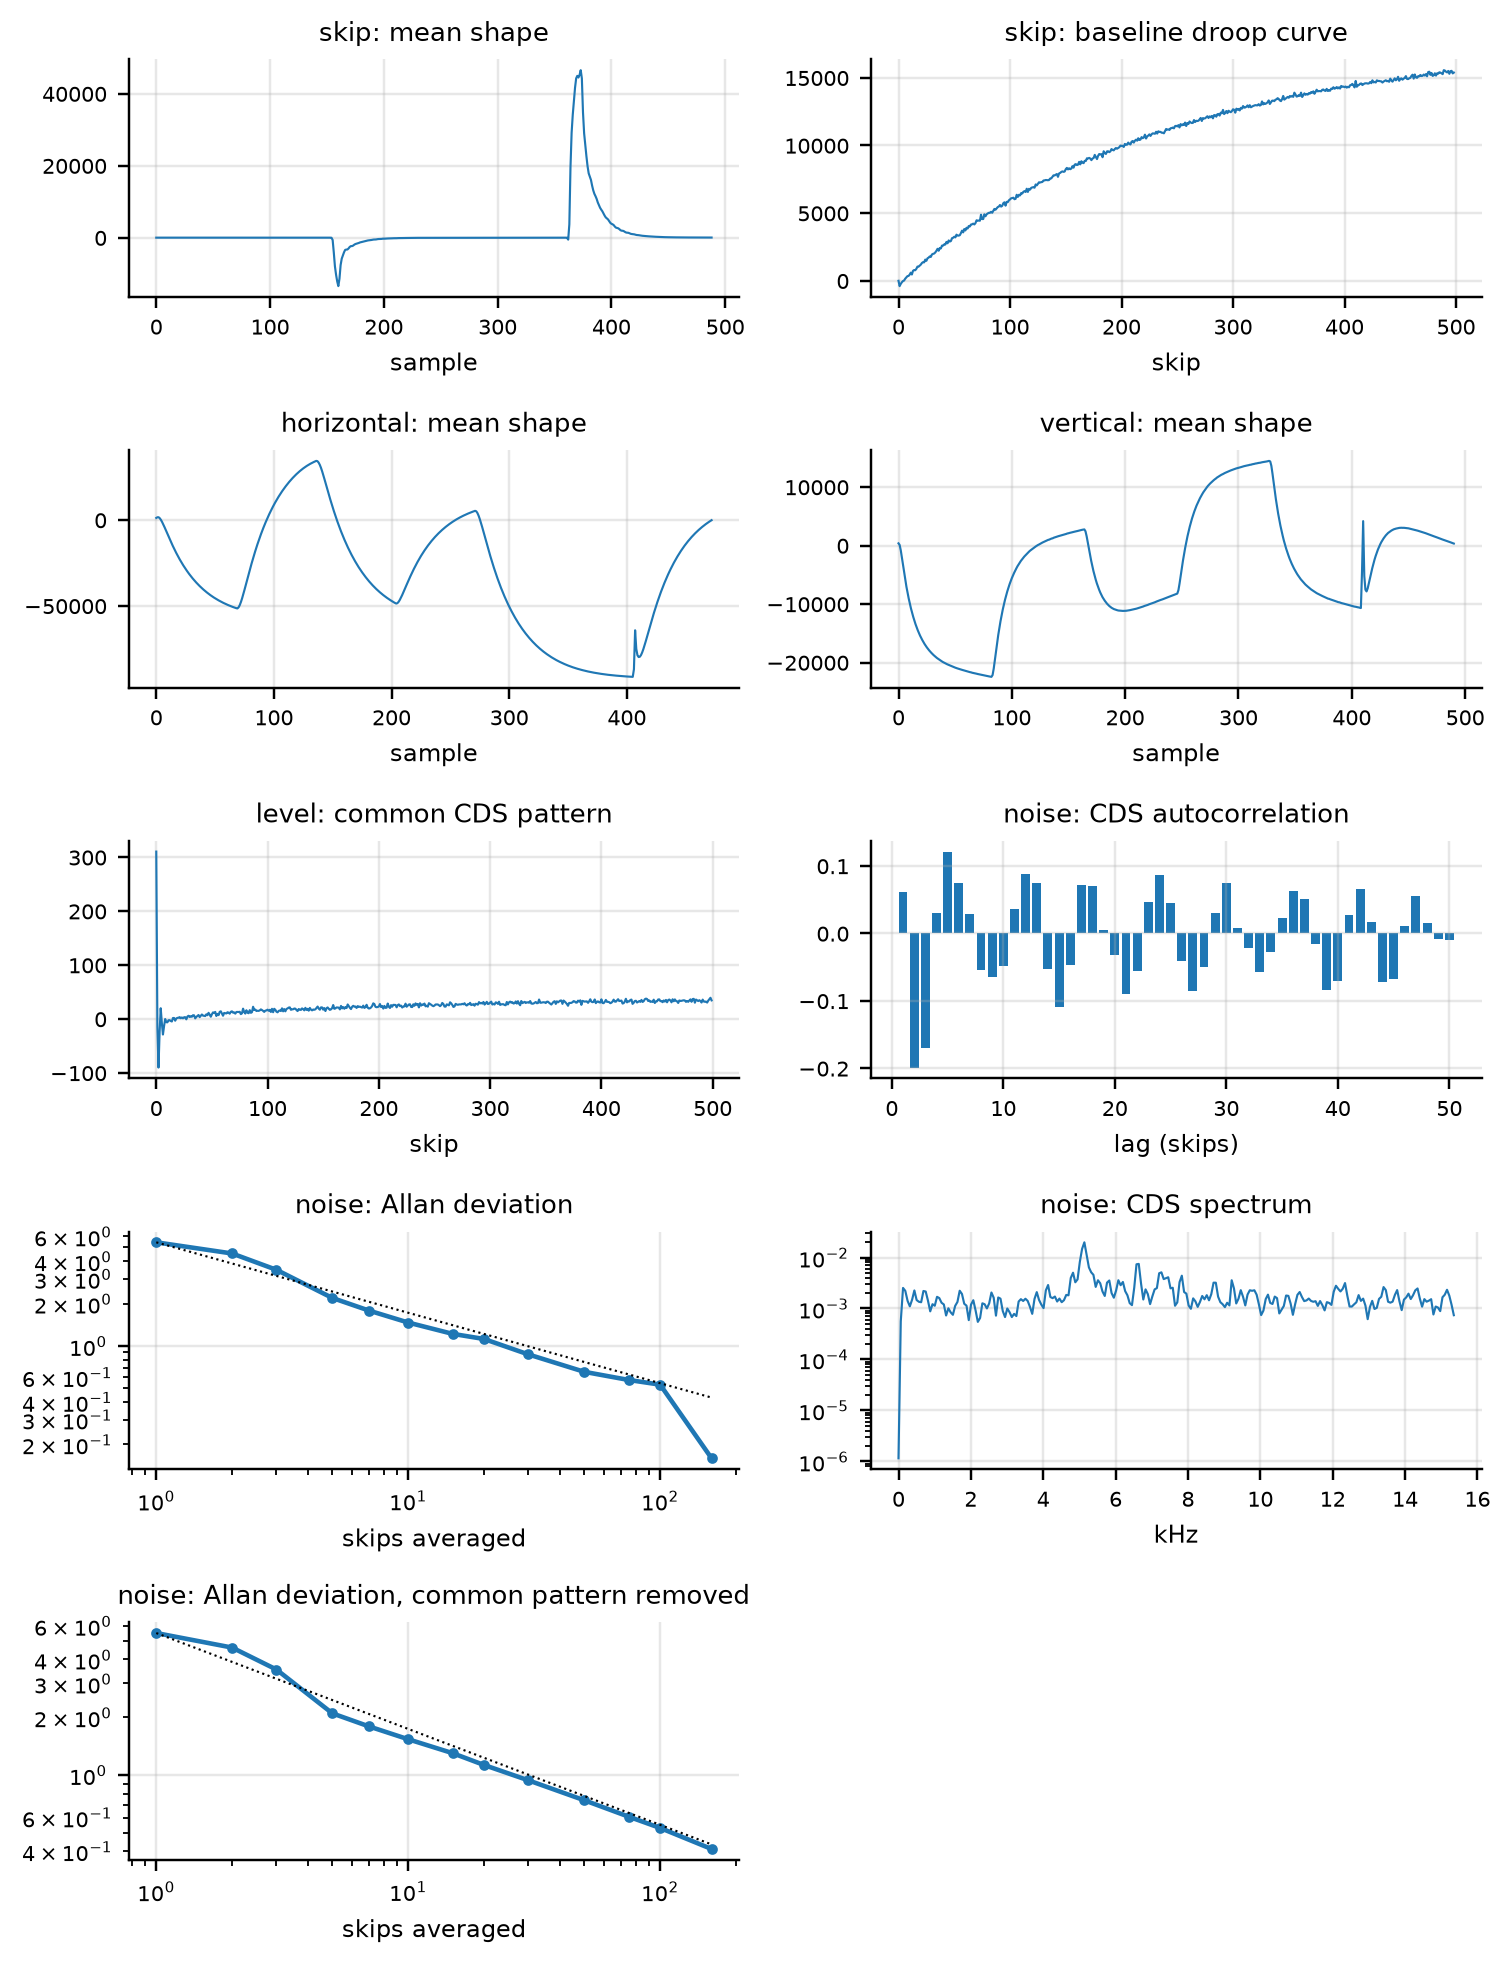
\includegraphics[width=1.0\textwidth,height=0.78\textheight,keepaspectratio]{all_curves_a.png}
\caption{The 18 curves returned by trace\_features, part 1 of 2. Example trace: module 101, channel 0, 2026-10-08, first repeat.}
\label{fig:all_curves_a}
\end{figure}

\begin{figure}[htbp]
\centering
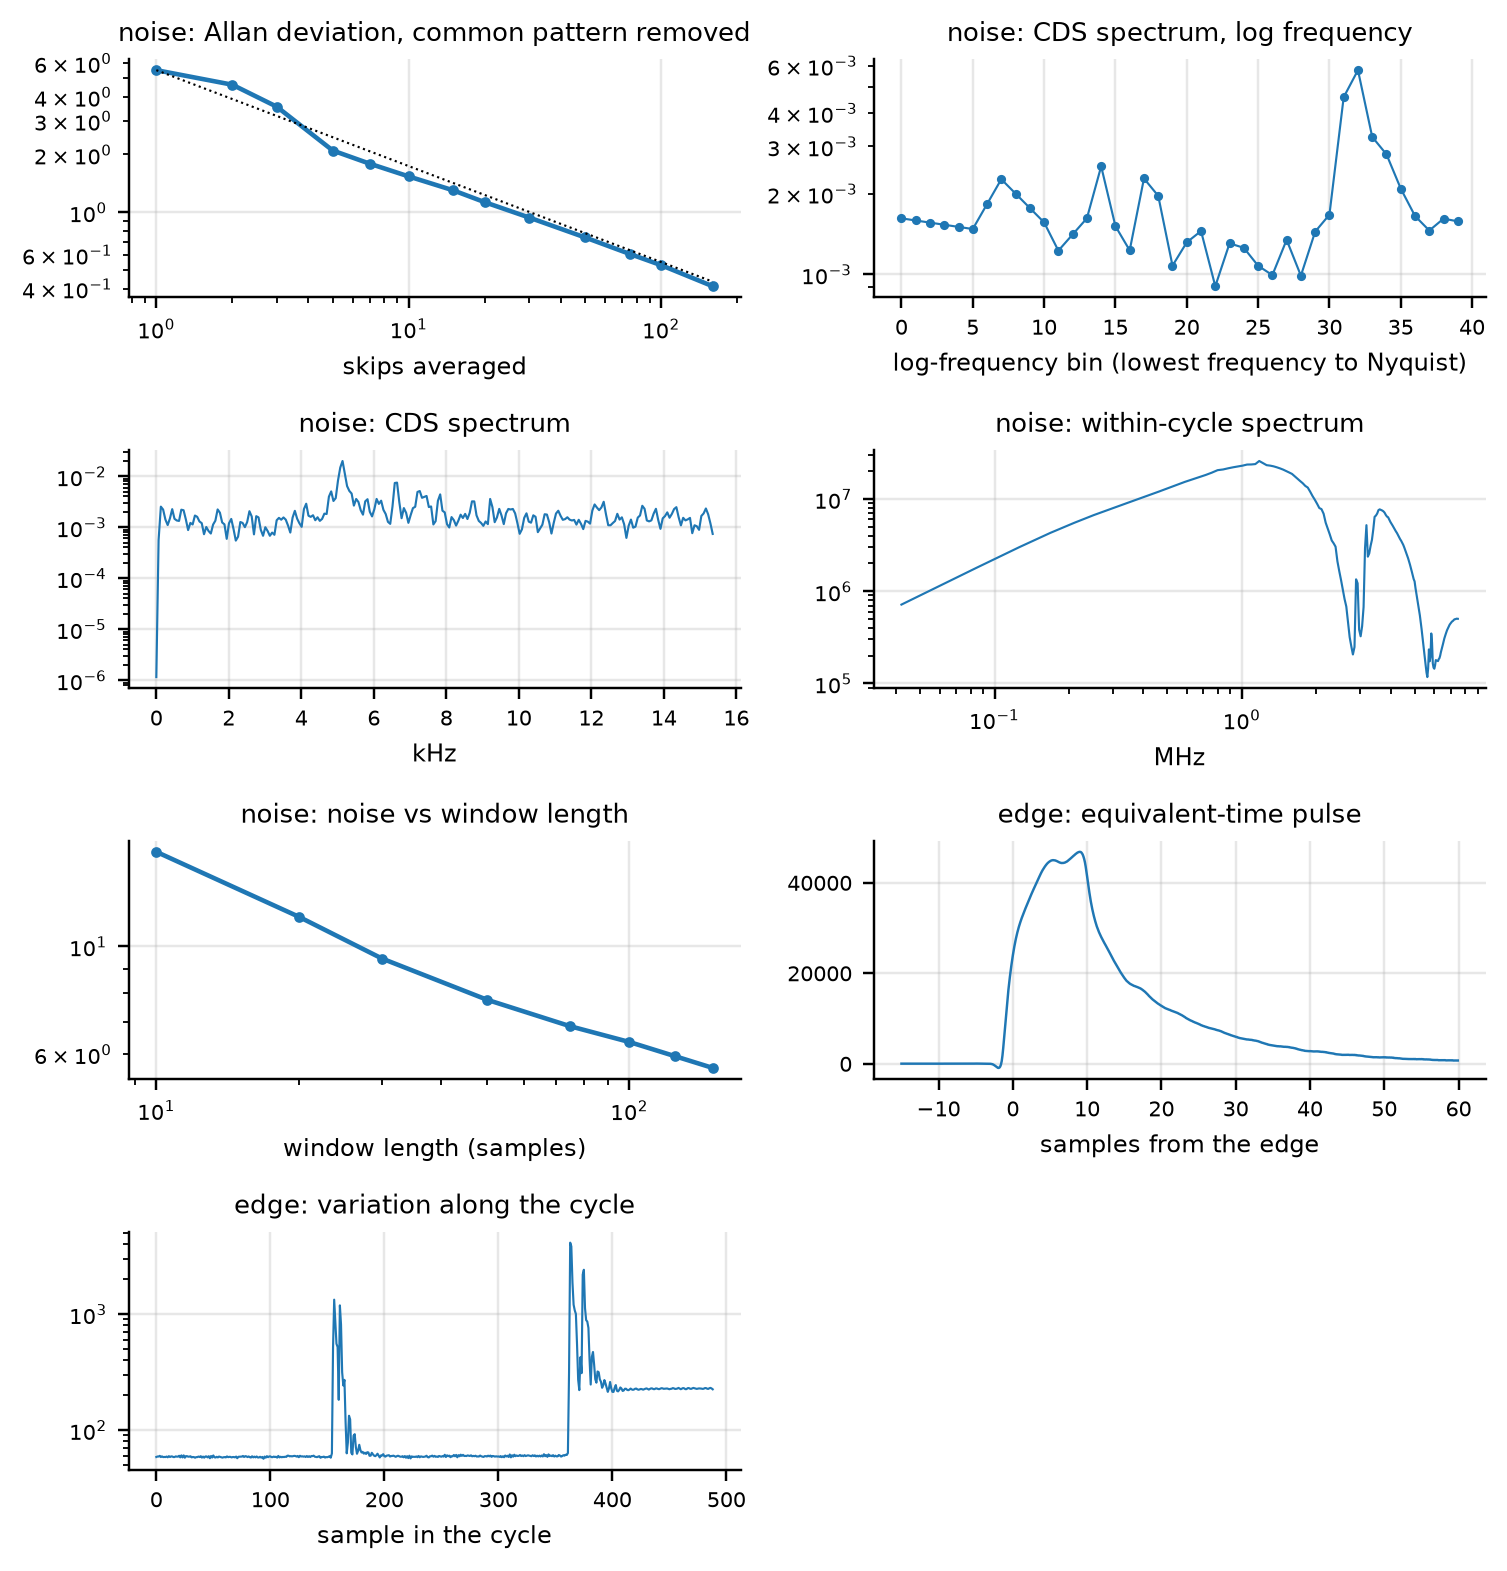
\includegraphics[width=1.0\textwidth,height=0.78\textheight,keepaspectratio]{all_curves_b.png}
\caption{The 18 curves returned by trace\_features, part 2 of 2. Example trace: module 101, channel 0, 2026-10-08, first repeat.}
\label{fig:all_curves_b}
\end{figure}

\clearpage


\section{Which features separate amplifiers better than repeats}

On the 2026-10-08 session (module 101, 19 healthy traces: 4 channels $\times$ 5 repeats, minus one
damaged trace), every feature was computed and, for each of the 6 pairs of channels,
\begin{equation}
\text{separation} = \frac{|\overline{f}_A-\overline{f}_B|}{s_\text{pooled}},
\end{equation}
where $s_\text{pooled}$ is the pooled standard deviation of the repeats. A separation of at least 3 means the feature tells two
amplifiers apart well beyond its repeat scatter: the precondition for seeing a change of the operating parameters. Features with a
zero repeat scatter would give an undefined separation (shown as --); a pair in which both amplifiers have zero scatter is left
out of the median (e.g.\ the in-window step rate, which is exactly 0 on every amplifier but ch2).
25 features separate all 6 pairs and 50 separate none.
A low separation does not make a feature useless: a feature that is the same on every amplifier (e.g.\ the baseline coupling) is
a clean parameter signal if it moves with $\theta$. Only a scan with varied parameters can show which features respond to $\theta$
and to the image labels.

\begin{figure}[p]
\centering
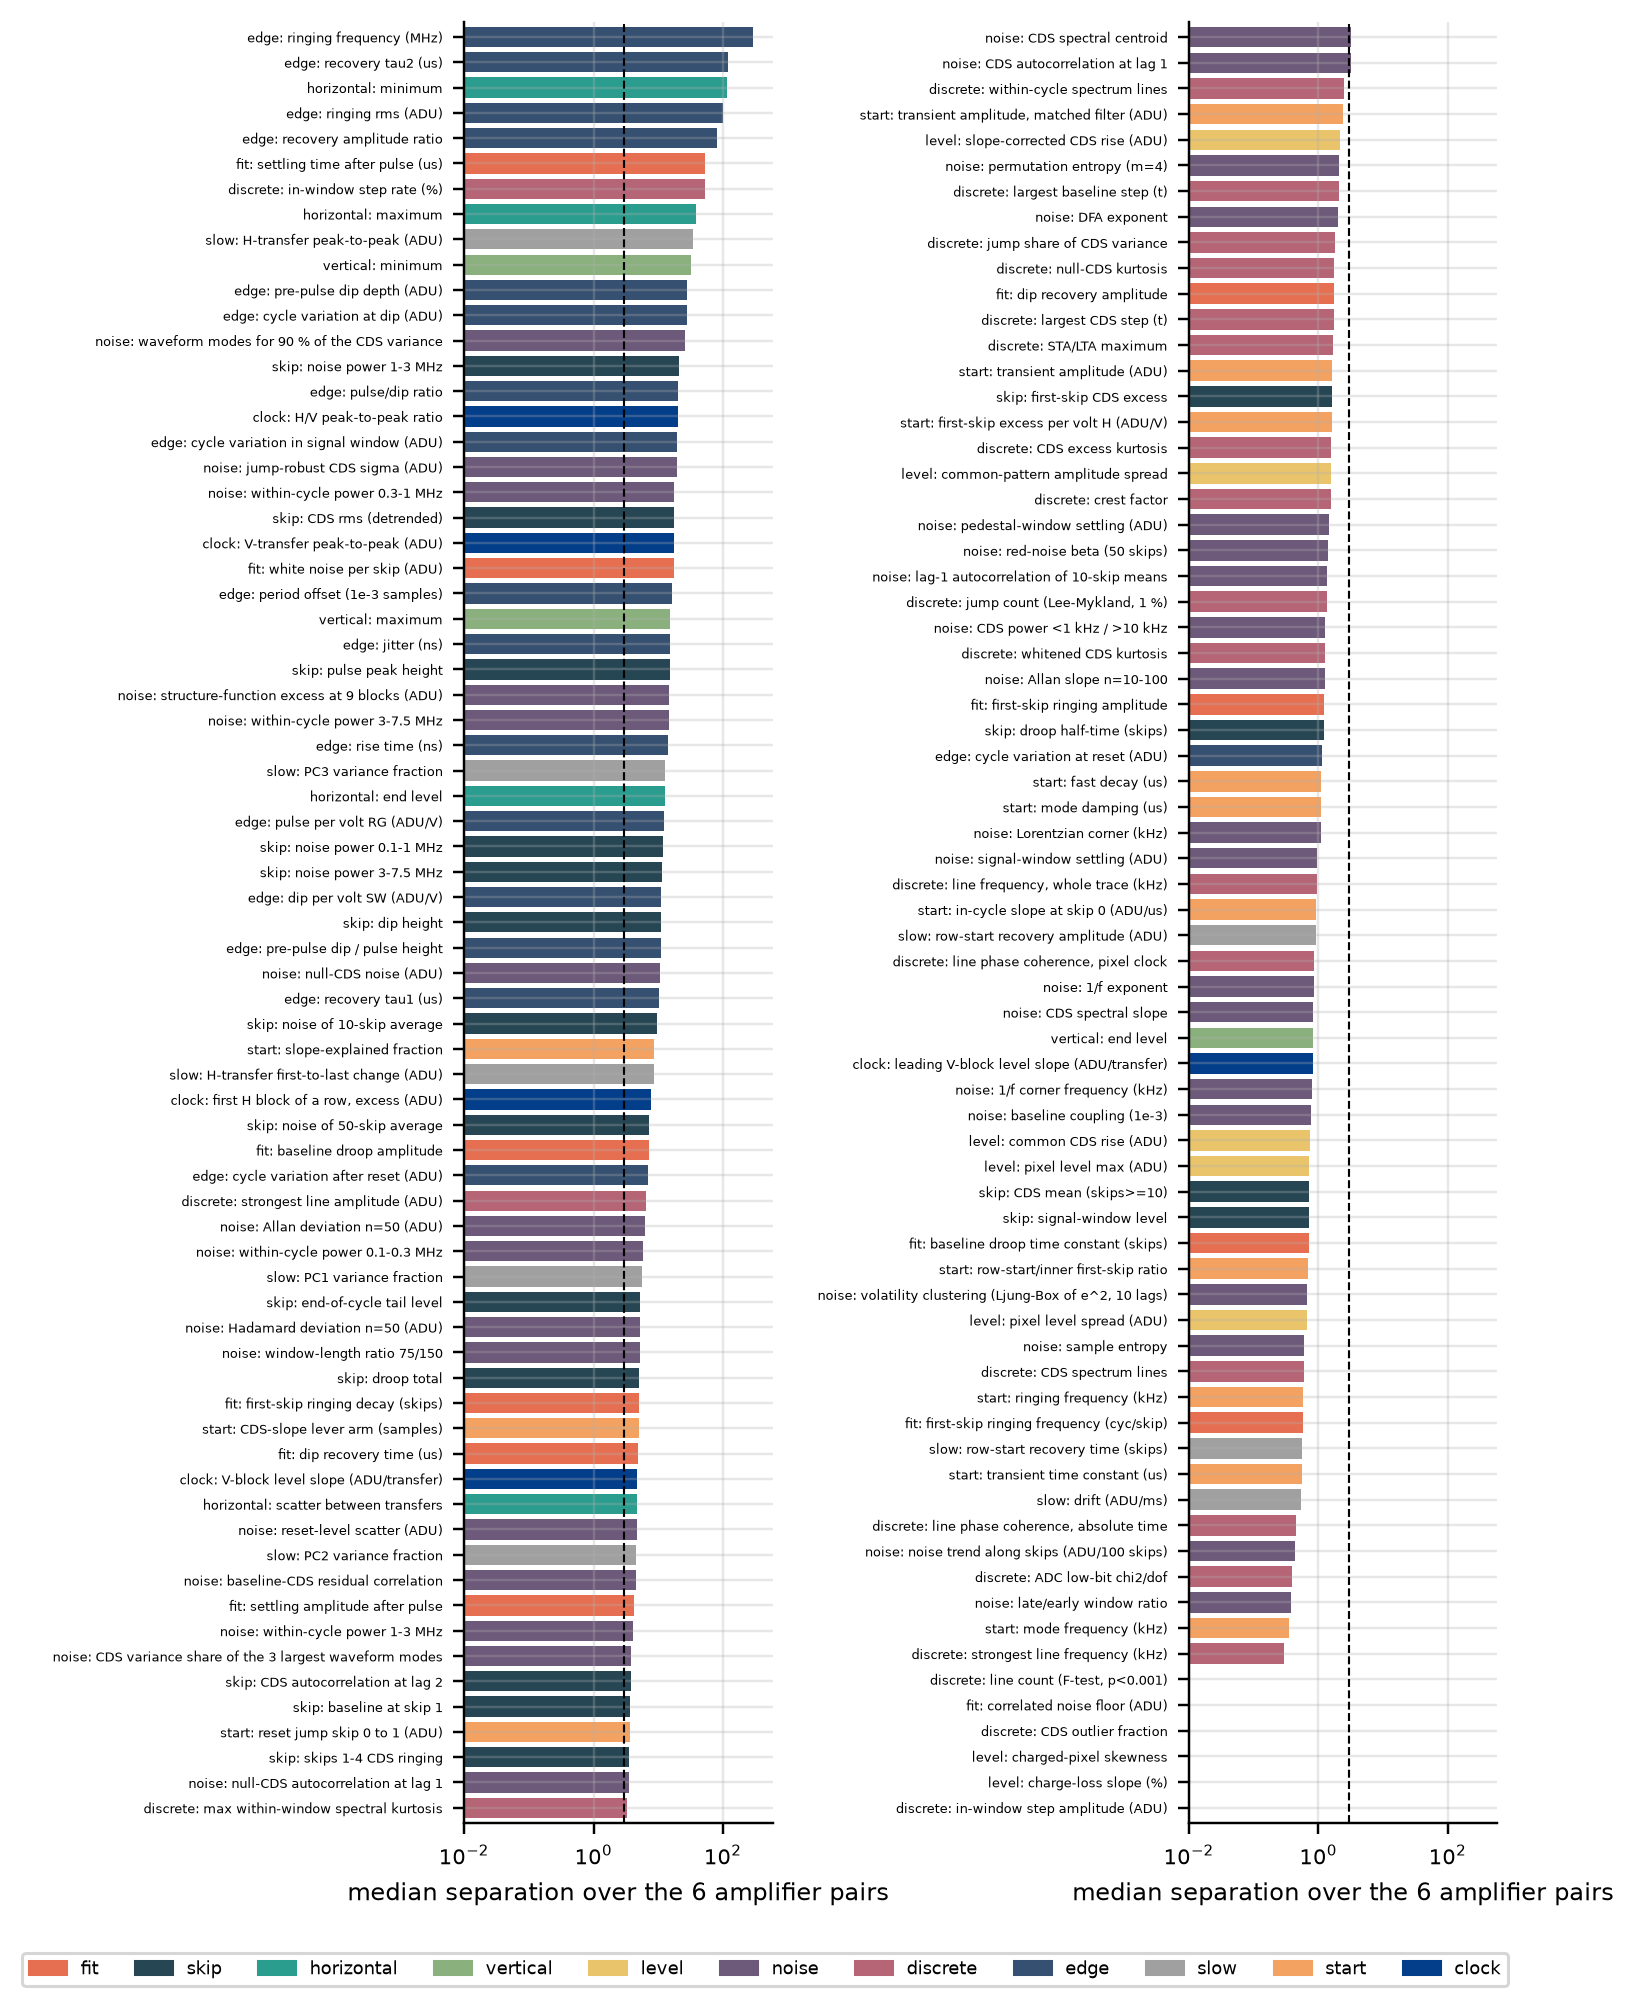
\includegraphics[width=1.0\textwidth,height=0.78\textheight,keepaspectratio]{feature_separation.png}
\caption{Median separation over the 6 channel pairs (difference of the means divided by the pooled repeat scatter), coloured by group; dashed line: 3.}
\label{fig:feature_separation}
\end{figure}

\clearpage

\begin{longtable}{>{\raggedright\arraybackslash}p{0.55\textwidth}rr}
\toprule Feature & Pairs $\geq 3$ & Median separation \\ \midrule \endhead
\bottomrule \endfoot
\texttt{edge: ringing frequency (MHz)} & 6 & 293.3 \\
\texttt{edge: recovery tau2 (us)} & 6 & 120.4 \\
\texttt{horizontal: minimum} & 6 & 114.4 \\
\texttt{edge: ringing rms (ADU)} & 6 & 99.1 \\
\texttt{edge: recovery amplitude ratio} & 6 & 79.9 \\
\texttt{fit: settling time after pulse (us)} & 6 & 52.8 \\
\texttt{discrete: in-window step rate (\%)} & 3 & 52.4 \\
\texttt{horizontal: maximum} & 6 & 38.1 \\
\texttt{slow: H-transfer peak-to-peak (ADU)} & 6 & 34.4 \\
\texttt{vertical: minimum} & 6 & 31.6 \\
\texttt{edge: pre-pulse dip depth (ADU)} & 6 & 28.2 \\
\texttt{edge: cycle variation at dip (ADU)} & 6 & 27.6 \\
\texttt{noise: waveform modes for 90 \% of the CDS variance} & 6 & 26.4 \\
\texttt{skip: noise power 1-3 MHz} & 6 & 21.0 \\
\texttt{edge: pulse/dip ratio} & 6 & 20.1 \\
\texttt{clock: H/V peak-to-peak ratio} & 6 & 20.0 \\
\texttt{edge: cycle variation in signal window (ADU)} & 6 & 19.5 \\
\texttt{noise: jump-robust CDS sigma (ADU)} & 5 & 19.2 \\
\texttt{noise: within-cycle power 0.3-1 MHz} & 5 & 17.8 \\
\texttt{skip: CDS rms (detrended)} & 5 & 17.6 \\
\texttt{clock: V-transfer peak-to-peak (ADU)} & 6 & 17.4 \\
\texttt{fit: white noise per skip (ADU)} & 5 & 17.3 \\
\texttt{edge: period offset (1e-3 samples)} & 5 & 16.3 \\
\texttt{vertical: maximum} & 6 & 15.4 \\
\texttt{edge: jitter (ns)} & 4 & 15.4 \\
\texttt{skip: pulse peak height} & 5 & 15.3 \\
\texttt{noise: structure-function excess at 9 blocks (ADU)} & 6 & 14.6 \\
\texttt{noise: within-cycle power 3-7.5 MHz} & 6 & 14.6 \\
\texttt{edge: rise time (ns)} & 4 & 14.0 \\
\texttt{slow: PC3 variance fraction} & 3 & 12.6 \\
\texttt{horizontal: end level} & 4 & 12.6 \\
\texttt{edge: pulse per volt RG (ADU/V)} & 6 & 12.2 \\
\texttt{skip: noise power 0.1-1 MHz} & 3 & 12.0 \\
\texttt{skip: noise power 3-7.5 MHz} & 5 & 11.5 \\
\texttt{edge: dip per volt SW (ADU/V)} & 5 & 11.0 \\
\texttt{skip: dip height} & 5 & 10.9 \\
\texttt{edge: pre-pulse dip / pulse height} & 6 & 10.9 \\
\texttt{noise: null-CDS noise (ADU)} & 6 & 10.5 \\
\texttt{edge: recovery tau1 (us)} & 6 & 10.4 \\
\texttt{skip: noise of 10-skip average} & 6 & 9.5 \\
\texttt{start: slope-explained fraction} & 4 & 8.6 \\
\texttt{slow: H-transfer first-to-last change (ADU)} & 5 & 8.5 \\
\texttt{clock: first H block of a row, excess (ADU)} & 5 & 7.6 \\
\texttt{skip: noise of 50-skip average} & 4 & 7.1 \\
\texttt{fit: baseline droop amplitude} & 5 & 7.1 \\
\texttt{edge: cycle variation after reset (ADU)} & 4 & 6.9 \\
\texttt{discrete: strongest line amplitude (ADU)} & 3 & 6.4 \\
\texttt{noise: Allan deviation n=50 (ADU)} & 4 & 6.3 \\
\texttt{noise: within-cycle power 0.1-0.3 MHz} & 5 & 5.8 \\
\texttt{slow: PC1 variance fraction} & 4 & 5.5 \\
\texttt{skip: end-of-cycle tail level} & 4 & 5.3 \\
\texttt{noise: Hadamard deviation n=50 (ADU)} & 4 & 5.2 \\
\texttt{noise: window-length ratio 75/150} & 5 & 5.1 \\
\texttt{skip: droop total} & 5 & 5.1 \\
\texttt{fit: first-skip ringing decay (skips)} & 3 & 5.0 \\
\texttt{start: CDS-slope lever arm (samples)} & 3 & 5.0 \\
\texttt{fit: dip recovery time (us)} & 5 & 5.0 \\
\texttt{clock: V-block level slope (ADU/transfer)} & 5 & 4.8 \\
\texttt{horizontal: scatter between transfers} & 5 & 4.7 \\
\texttt{noise: reset-level scatter (ADU)} & 3 & 4.7 \\
\texttt{slow: PC2 variance fraction} & 4 & 4.6 \\
\texttt{noise: baseline-CDS residual correlation} & 3 & 4.5 \\
\texttt{fit: settling amplitude after pulse} & 4 & 4.2 \\
\texttt{noise: within-cycle power 1-3 MHz} & 3 & 4.0 \\
\texttt{noise: CDS variance share of the 3 largest waveform modes} & 3 & 3.8 \\
\texttt{skip: CDS autocorrelation at lag 2} & 3 & 3.7 \\
\texttt{skip: baseline at skip 1} & 3 & 3.7 \\
\texttt{start: reset jump skip 0 to 1 (ADU)} & 3 & 3.7 \\
\texttt{skip: skips 1-4 CDS ringing} & 3 & 3.5 \\
\texttt{noise: null-CDS autocorrelation at lag 1} & 4 & 3.5 \\
\texttt{discrete: max within-window spectral kurtosis} & 3 & 3.3 \\
\texttt{noise: CDS spectral centroid} & 3 & 3.2 \\
\texttt{noise: CDS autocorrelation at lag 1} & 3 & 3.2 \\
\texttt{discrete: within-cycle spectrum lines} & 0 & 2.5 \\
\texttt{start: transient amplitude, matched filter (ADU)} & 2 & 2.4 \\
\texttt{level: slope-corrected CDS rise (ADU)} & 0 & 2.1 \\
\texttt{noise: permutation entropy (m=4)} & 1 & 2.1 \\
\texttt{discrete: largest baseline step (t)} & 3 & 2.1 \\
\texttt{noise: DFA exponent} & 2 & 2.0 \\
\texttt{discrete: jump share of CDS variance} & 1 & 1.8 \\
\texttt{discrete: null-CDS kurtosis} & 0 & 1.8 \\
\texttt{fit: dip recovery amplitude} & 2 & 1.7 \\
\texttt{discrete: largest CDS step (t)} & 0 & 1.7 \\
\texttt{discrete: STA/LTA maximum} & 1 & 1.7 \\
\texttt{start: transient amplitude (ADU)} & 2 & 1.7 \\
\texttt{skip: first-skip CDS excess} & 2 & 1.6 \\
\texttt{start: first-skip excess per volt H (ADU/V)} & 2 & 1.6 \\
\texttt{discrete: CDS excess kurtosis} & 0 & 1.6 \\
\texttt{level: common-pattern amplitude spread} & 0 & 1.6 \\
\texttt{discrete: crest factor} & 0 & 1.5 \\
\texttt{noise: pedestal-window settling (ADU)} & 2 & 1.5 \\
\texttt{noise: red-noise beta (50 skips)} & 0 & 1.4 \\
\texttt{noise: lag-1 autocorrelation of 10-skip means} & 1 & 1.4 \\
\texttt{discrete: jump count (Lee-Mykland, 1 \%)} & 0 & 1.4 \\
\texttt{noise: CDS power \textless{}1 kHz / \textgreater{}10 kHz} & 0 & 1.3 \\
\texttt{discrete: whitened CDS kurtosis} & 0 & 1.3 \\
\texttt{noise: Allan slope n=10-100} & 0 & 1.2 \\
\texttt{fit: first-skip ringing amplitude} & 1 & 1.2 \\
\texttt{skip: droop half-time (skips)} & 0 & 1.2 \\
\texttt{edge: cycle variation at reset (ADU)} & 0 & 1.1 \\
\texttt{start: fast decay (us)} & 0 & 1.1 \\
\texttt{start: mode damping (us)} & 0 & 1.1 \\
\texttt{noise: Lorentzian corner (kHz)} & 0 & 1.1 \\
\texttt{noise: signal-window settling (ADU)} & 0 & 1.0 \\
\texttt{discrete: line frequency, whole trace (kHz)} & 0 & 1.0 \\
\texttt{start: in-cycle slope at skip 0 (ADU/us)} & 2 & 0.9 \\
\texttt{slow: row-start recovery amplitude (ADU)} & 1 & 0.9 \\
\texttt{discrete: line phase coherence, pixel clock} & 0 & 0.9 \\
\texttt{noise: 1/f exponent} & 0 & 0.8 \\
\texttt{noise: CDS spectral slope} & 0 & 0.8 \\
\texttt{vertical: end level} & 1 & 0.8 \\
\texttt{clock: leading V-block level slope (ADU/transfer)} & 0 & 0.8 \\
\texttt{noise: 1/f corner frequency (kHz)} & 0 & 0.8 \\
\texttt{noise: baseline coupling (1e-3)} & 0 & 0.8 \\
\texttt{level: common CDS rise (ADU)} & 1 & 0.7 \\
\texttt{level: pixel level max (ADU)} & 0 & 0.7 \\
\texttt{skip: CDS mean (skips\textgreater{}=10)} & 0 & 0.7 \\
\texttt{skip: signal-window level} & 0 & 0.7 \\
\texttt{fit: baseline droop time constant (skips)} & 2 & 0.7 \\
\texttt{start: row-start/inner first-skip ratio} & 0 & 0.7 \\
\texttt{noise: volatility clustering (Ljung-Box of e\textasciicircum{}2, 10 lags)} & 0 & 0.7 \\
\texttt{level: pixel level spread (ADU)} & 0 & 0.7 \\
\texttt{noise: sample entropy} & 0 & 0.6 \\
\texttt{discrete: CDS spectrum lines} & 0 & 0.6 \\
\texttt{start: ringing frequency (kHz)} & 0 & 0.6 \\
\texttt{fit: first-skip ringing frequency (cyc/skip)} & 0 & 0.6 \\
\texttt{slow: row-start recovery time (skips)} & 0 & 0.6 \\
\texttt{start: transient time constant (us)} & 0 & 0.6 \\
\texttt{slow: drift (ADU/ms)} & 0 & 0.5 \\
\texttt{discrete: line phase coherence, absolute time} & 0 & 0.5 \\
\texttt{noise: noise trend along skips (ADU/100 skips)} & 0 & 0.4 \\
\texttt{discrete: ADC low-bit chi2/dof} & 0 & 0.4 \\
\texttt{noise: late/early window ratio} & 0 & 0.4 \\
\texttt{start: mode frequency (kHz)} & 0 & 0.3 \\
\texttt{discrete: strongest line frequency (kHz)} & 0 & 0.3 \\
\texttt{discrete: line count (F-test, p\textless{}0.001)} & 0 & -- \\
\texttt{fit: correlated noise floor (ADU)} & 0 & -- \\
\texttt{discrete: CDS outlier fraction} & 0 & -- \\
\texttt{level: charged-pixel skewness} & 0 & -- \\
\texttt{level: charge-loss slope (\%)} & 0 & -- \\
\texttt{discrete: in-window step amplitude (ADU)} & 0 & -- \\
\end{longtable}

\section{Nearly redundant features}

Pairs of features whose values are correlated with $|r|>0.98$ across the same 19 traces (189 pairs;
the 30 strongest are listed). With 19 traces from 4 amplifiers, such correlations mostly mean that both features follow the same
amplifier difference; they suggest redundancy, but only a parameter scan shows whether they also move together with $\theta$.
Some pairs are redundant by construction (e.g.\ the signal-window level and the CDS mean; the dip height and the dip per volt at a
fixed swing).

\begin{figure}[p]
\centering
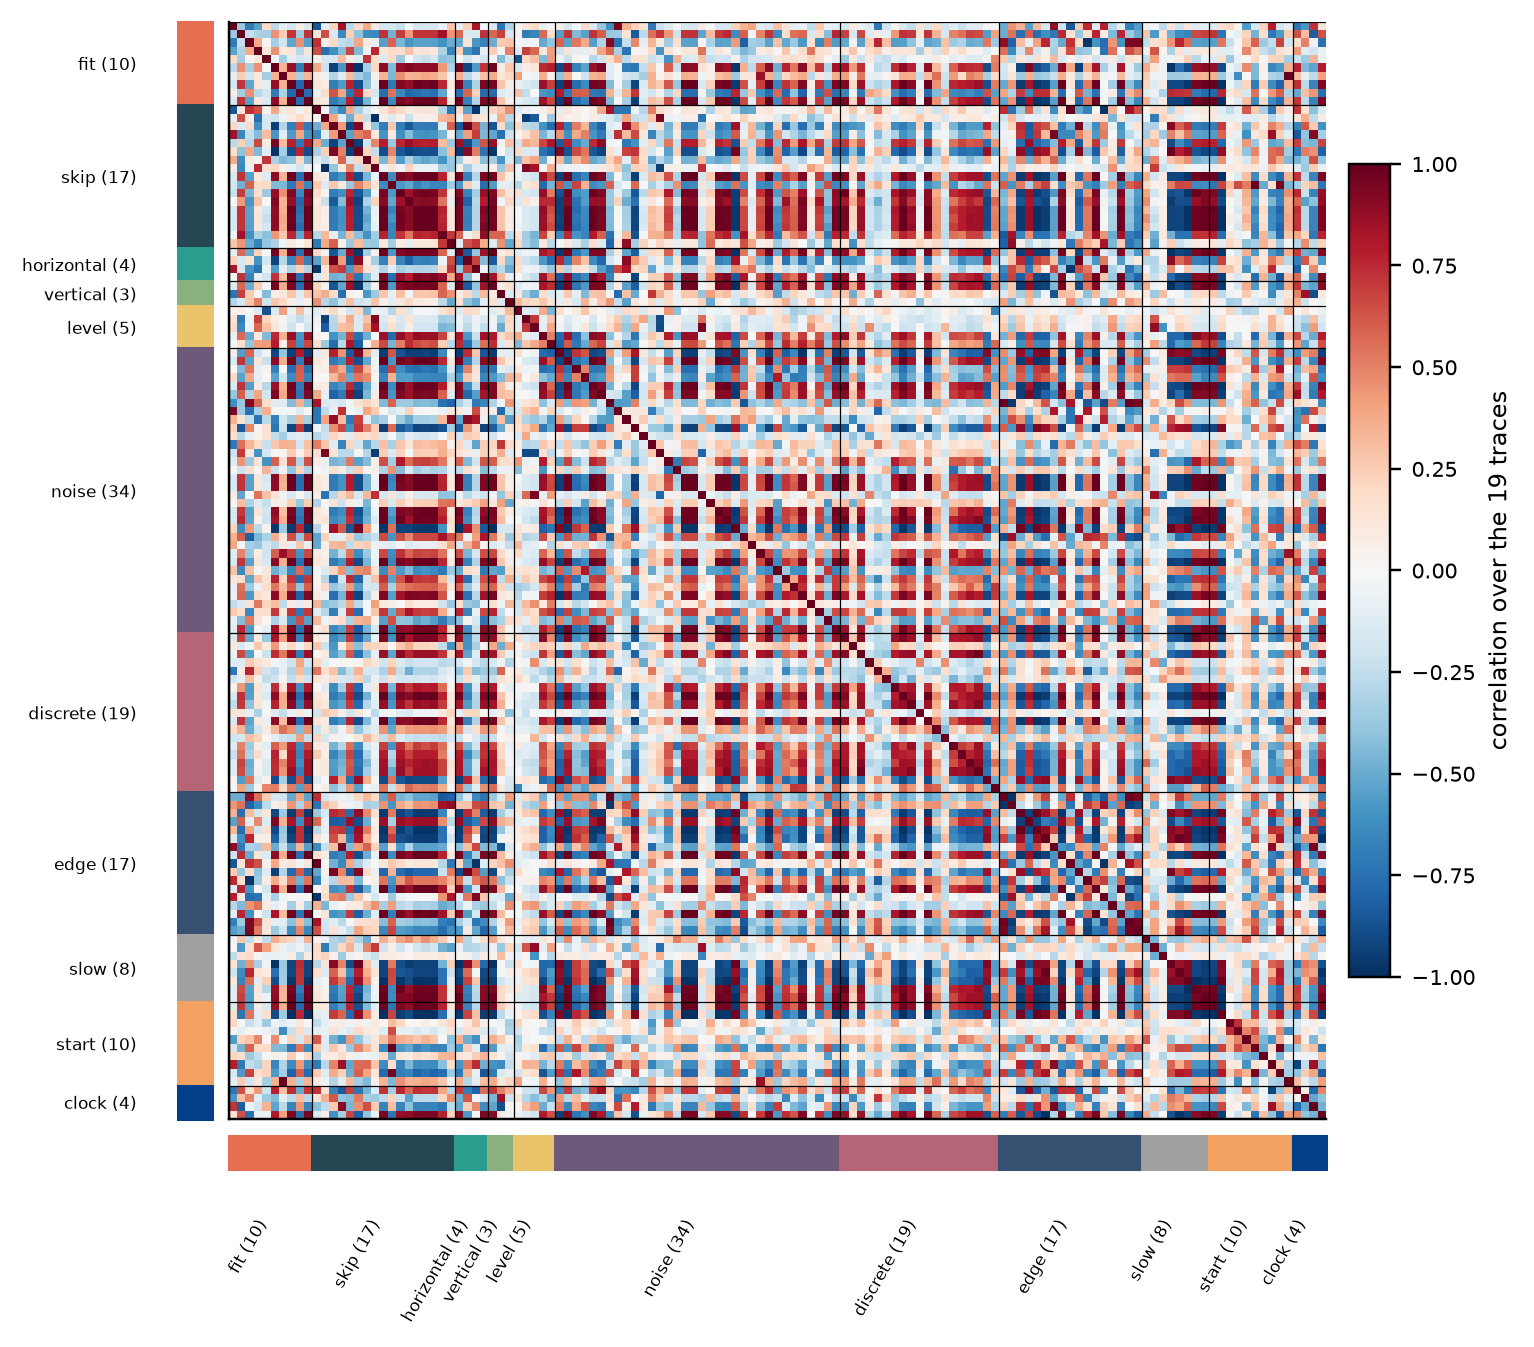
\includegraphics[width=1.0\textwidth,height=0.78\textheight,keepaspectratio]{feature_correlation.png}
\caption{Correlation between the features across the 19 healthy traces of the 2026-10-08 session (features that are NaN in any trace, or constant, are left out), grouped by feature group, in registry order within a group (the bands show the groups and how many features each has). The strongest individual pairs are listed in the table below.}
\label{fig:feature_correlation}
\end{figure}

\clearpage

\begin{longtable}{>{\raggedright\arraybackslash}p{0.40\textwidth}>{\raggedright\arraybackslash}p{0.40\textwidth}r}
\toprule Feature & Feature & $r$ \\ \midrule \endhead
\bottomrule \endfoot
\texttt{fit: first-skip ringing frequency (cyc/skip)} & \texttt{start: ringing frequency (kHz)} & +1.000 \\
\texttt{skip: first-skip CDS excess} & \texttt{start: first-skip excess per volt H (ADU/V)} & +1.000 \\
\texttt{skip: signal-window level} & \texttt{skip: CDS mean (skips\textgreater{}=10)} & -1.000 \\
\texttt{skip: dip height} & \texttt{edge: dip per volt SW (ADU/V)} & +1.000 \\
\texttt{fit: white noise per skip (ADU)} & \texttt{skip: CDS rms (detrended)} & +1.000 \\
\texttt{fit: white noise per skip (ADU)} & \texttt{noise: jump-robust CDS sigma (ADU)} & +1.000 \\
\texttt{skip: CDS rms (detrended)} & \texttt{noise: jump-robust CDS sigma (ADU)} & +1.000 \\
\texttt{skip: noise of 10-skip average} & \texttt{noise: null-CDS noise (ADU)} & +1.000 \\
\texttt{skip: noise of 10-skip average} & \texttt{noise: structure-function excess at 9 blocks (ADU)} & +0.999 \\
\texttt{start: slope-explained fraction} & \texttt{noise: structure-function excess at 9 blocks (ADU)} & -0.999 \\
\texttt{discrete: in-window step rate (\%)} & \texttt{noise: jump-robust CDS sigma (ADU)} & +0.999 \\
\texttt{skip: noise power 0.1-1 MHz} & \texttt{noise: structure-function excess at 9 blocks (ADU)} & +0.999 \\
\texttt{noise: null-CDS noise (ADU)} & \texttt{noise: structure-function excess at 9 blocks (ADU)} & +0.999 \\
\texttt{skip: noise power 0.1-1 MHz} & \texttt{discrete: in-window step rate (\%)} & +0.999 \\
\texttt{fit: white noise per skip (ADU)} & \texttt{noise: structure-function excess at 9 blocks (ADU)} & +0.999 \\
\texttt{skip: CDS rms (detrended)} & \texttt{discrete: in-window step rate (\%)} & +0.999 \\
\texttt{fit: white noise per skip (ADU)} & \texttt{discrete: in-window step rate (\%)} & +0.999 \\
\texttt{skip: CDS rms (detrended)} & \texttt{noise: structure-function excess at 9 blocks (ADU)} & +0.999 \\
\texttt{skip: noise power 0.1-1 MHz} & \texttt{noise: jump-robust CDS sigma (ADU)} & +0.999 \\
\texttt{horizontal: minimum} & \texttt{vertical: minimum} & +0.999 \\
\texttt{skip: CDS rms (detrended)} & \texttt{skip: noise power 0.1-1 MHz} & +0.999 \\
\texttt{noise: jump-robust CDS sigma (ADU)} & \texttt{noise: structure-function excess at 9 blocks (ADU)} & +0.999 \\
\texttt{fit: white noise per skip (ADU)} & \texttt{skip: noise power 0.1-1 MHz} & +0.999 \\
\texttt{skip: noise of 10-skip average} & \texttt{start: slope-explained fraction} & -0.999 \\
\texttt{skip: noise of 10-skip average} & \texttt{skip: noise power 0.1-1 MHz} & +0.999 \\
\texttt{skip: noise power 0.1-1 MHz} & \texttt{noise: null-CDS noise (ADU)} & +0.999 \\
\texttt{start: slope-explained fraction} & \texttt{noise: null-CDS noise (ADU)} & -0.999 \\
\texttt{skip: noise of 50-skip average} & \texttt{noise: Allan deviation n=50 (ADU)} & +0.999 \\
\texttt{discrete: in-window step rate (\%)} & \texttt{noise: structure-function excess at 9 blocks (ADU)} & +0.999 \\
\texttt{edge: ringing rms (ADU)} & \texttt{discrete: in-window step rate (\%)} & +0.998 \\
\end{longtable}

\section{Where it lives}
\begin{center}
\begin{tabular}{ll}
\toprule
Item & File \\
\midrule
Feature function and registry & \code{src/trace\_features.py} \\
The 2026-10-21 additions & \code{src/trace\_features\_extra.py} (registry \code{EXTRA}) \\
Tests of the additions & \code{tests/test\_trace\_features\_new.py} \\
Evidence tiers & \code{lvl1/feature\_study.py} $\to$ \code{lvl1/feature\_study/} \\
Learned tiers & \code{lvl1/feature\_importance.py} \\
Feature sets in training & \code{lvl1/train\_lvl1.py} (\code{--feature-tiers}, \code{--feature-ladder}) \\
Walkthrough of the additions & \code{lvl1/new\_trace\_features.ipynb} \\
Results of the additions & \code{docs/overleaf\_feature\_tiers\_2026-10-21} \\
Exact definitions & \code{docs/overleaf\_trace\_features\_technical} \\
Comparison tools (unchanged) & \code{src/compare\_trace.py} \\
Use in the pipeline & \code{src/process\_packet.py} (\code{process\_trace}) \\
Walkthrough of the merged set & \code{notebooks/trace\_features\_walkthrough.ipynb} \\
Development of the advanced features & \code{notebooks/advanced\_trace\_features.ipynb} \\
Description of the comparison tools & \code{docs/trace\_fit\_tools.tex} \\
\bottomrule
\end{tabular}
\end{center}

\end{document}
